\documentclass[11pt]{article}
\usepackage[margin=1in]{geometry}
\usepackage{amsmath,amssymb}
\usepackage{booktabs}
\usepackage{enumitem}
\usepackage{tikz}
\usetikzlibrary{positioning,arrows.meta,fit}
\usepackage[table]{xcolor}
\usepackage[hidelinks]{hyperref}
\usepackage{graphicx}

% colour families: IO/data, policy, backbone/structure (teal), sequence (amber)
\definecolor{ioFill}{RGB}{237,242,247}\definecolor{ioLine}{RGB}{90,107,130}
\definecolor{lfFill}{RGB}{231,222,246}\definecolor{lfLine}{RGB}{108,63,176}
\definecolor{aFill}{RGB}{201,235,221}\definecolor{aLine}{RGB}{30,140,110}
\definecolor{bFill}{RGB}{251,227,196}\definecolor{bLine}{RGB}{200,122,30}
\definecolor{dFill}{RGB}{214,229,247}\definecolor{dLine}{RGB}{40,96,168}
\definecolor{aTint}{RGB}{233,247,241}\definecolor{bTint}{RGB}{252,242,229}
\definecolor{dTint}{RGB}{233,241,251}

\setlist{nosep,leftmargin=1.4em}
\setlength{\parindent}{0pt}
\setlength{\parskip}{0.4em}

\newcommand{\R}{\mathrm{R}}
\newcommand{\SC}{\mathrm{SC}}
\newcommand{\TV}{\mathrm{TV}}
\newcommand{\eclash}{E_{\mathrm{clash}}}
\newcommand{\ttk}[1]{\texttt{\small #1}}
\newcommand{\tabnote}[1]{\par\vspace{-0.15em}\noindent%
  \begin{minipage}{\linewidth}\footnotesize\itshape\raggedright
  \setlength{\emergencystretch}{2em}\sloppy #1\par\end{minipage}\par\vspace{0.5em}}

\begin{document}

\begin{center}
{\Large\bfseries The LeFlur GRPO reward stack:\\[2pt]
from a pre-trained binder policy to dense per-token rewards}\\[4pt]
{\normalsize LeFlur / LBSTER --- implementation note \quad$\cdot$\quad 2026-08-19}
\end{center}

\vspace{0.4em}

This note documents \emph{what is implemented and live}. It walks the pipeline in the order it
was built: (1) the pre-GRPO LeFlur binder policy and how it scores on the Complexa benchmark;
(2) how each decoded backbone is encoded into LigandMPNN to add side chains and a designed
sequence, which is the substrate for the rewards; (3) the distribution-based 3Di reward that
first realigned our interfaces; (4) the MPNN-based rewards; and (5) the current dense per-token
rewards. Every weight and knob quoted is from the live configs
\ttk{rl\_leflur\_binder\_grpo\_shape\_chord\_nodist\_accum10\_seqtrack} (HARD baseline) and its
per-token fork \ttk{...\_chord\_pertoken\_dist3di\_...}.

\section{The pre-GRPO LeFlur binder policy}
LeFlur is a multi-track discrete flow-matching (absorbing-state masked-diffusion) generator,
used here as the GRPO policy $\pi_\theta$ warm-started from \ttk{leflur-binder-3di}. It emits a
binder--target complex over three coupled tracks, all denoised jointly:
\begin{itemize}
\item \ttk{sequence} --- the binder amino-acid identities $a$;
\item \ttk{structure\_tokens} --- discrete backbone-geometry tokens $s$ (the fold);
\item \ttk{tri\_tokens} --- 3Di structural-alphabet tokens, capturing local backbone
  environment.
\end{itemize}
Generation is conditioned on the antigen target $T$ and a specified epitope $E$ (bidirectional
hotspot conditioning; epitope classifier-free guidance is the docking lever). A design is
produced by \ttk{rollout\_nsteps}$=40$ denoising steps; the benchmark uses the fold-diverse
inference schedule (\ttk{seq}=Power$^2$, \ttk{struc}=Linear, \ttk{tri}=Log) with the diversity
penalties that keep folds from collapsing.

\textbf{Benchmark standing (Complexa 38-target set, Protenix-scored).} Pre-GRPO LeFlur passes
$\approx\!10\text{--}13\%$ of designs (best arm $\approx\!12.9\%$), versus $\approx\!29\text{--}40\%$
for the Proteina-Complexa reference model --- a $\sim\!3\times$ gap. LeFlur also under-covers the
target set and is far less fold-diverse. Against de-novo baselines it ($\sim\!10\%$) trails
BoltzGen ($13\%$) and ESMFold2 ($12\%$) and beats PXDesign ($4\%$).

\begin{table}[htbp]
\centering
{\renewcommand{\arraystretch}{1.25}%
\begin{tabular}{@{}>{\raggedright\arraybackslash}p{6.4cm}
                    >{\centering\arraybackslash}p{3.1cm}
                    >{\centering\arraybackslash}p{3.4cm}@{}}
\toprule
\textbf{Complexa 38-target benchmark} & \textbf{LeFlur (pre-GRPO)} & \textbf{Proteina-Complexa}\\
\midrule
Protenix pass rate            & $\sim\!13\%$ & $\sim\!29\text{--}40\%$ \\
Target coverage               & $79\%$       & $100\%$ \\
Distinct folds / target       & $3.3$        & $11.5$ \\
\bottomrule
\end{tabular}}
\caption{The pre-GRPO starting point. Both models generate binders for the same $38$ Complexa
targets; \emph{Protenix pass rate} = fraction of designs whose Protenix-refolded complex clears the
acceptance filter, \emph{target coverage} = fraction of targets with $\geq\!1$ passing design,
\emph{distinct folds/target} = structural diversity of passing designs. Proteina-Complexa is the
external state-of-the-art model we are trying to close the gap to.}
\label{tab:benchmark}
\end{table}

\textbf{The diagnosed gaps} (what the reward stack targets):
\begin{itemize}
\item \emph{Shape-limited backbones.} On the hard PD1 target, rigid clash-gradient de-clash and
  post-hoc MPNN redesign both fail to transfer to Protenix; only a pose/shape change lifts
  interface 3DZD shape complementarity. The passing model sits at $\SC\!\approx\!0.956$ vs our
  $\approx\!0.918$ after every post-hoc fix --- the backbone \emph{shape at the epitope} is the
  lever.
\item \emph{Mis-aligned interface composition.} Native BindCraft/Complexa interfaces are
  V-dominated ($58\%/44\%$ 3Di) and fold-diverse; every LeFlur arm is D-heavy ($\sim\!20\text{--}27\%$)
  and monotonous. The Complexa model's interface distribution is closest to native (3Di TV
  $17.7\%$); ours is farthest.
\end{itemize}

\section{Encoding LeFlur backbones into LigandMPNN}
The rewards are not read off the raw tokens --- they are computed on an \emph{all-atom} complex.
Each decoded LeFlur backbone $X$ is handed to a frozen LigandMPNN, which
serves two products from a single round-trip:
a \textbf{pack} that adds side chains to the generated sequence, and a \textbf{design} that
re-predicts the sequence for that backbone.

\begin{center}
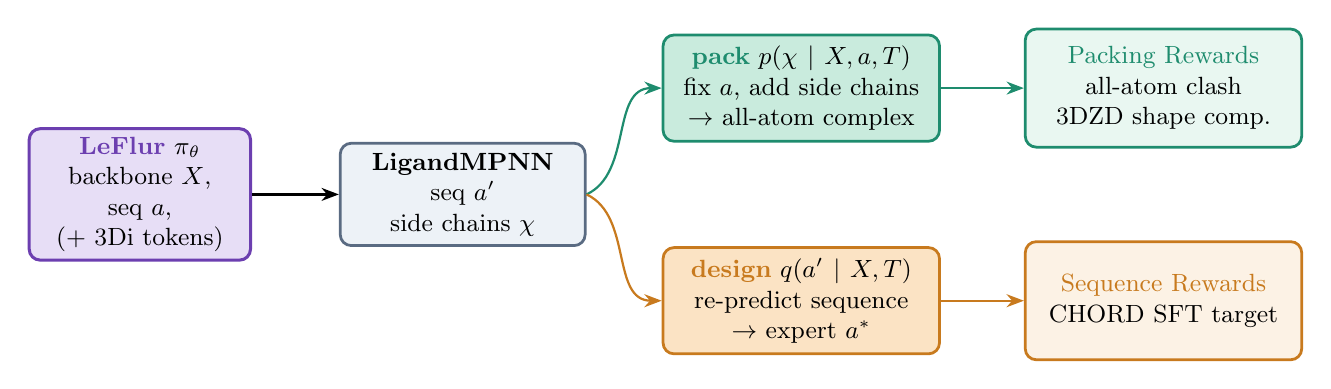
\begin{tikzpicture}[x=1cm,y=1cm,font=\small,>={Stealth[length=2.2mm]},
  io/.style  ={draw=ioLine,line width=0.9pt,rounded corners,align=center,text width=2.6cm,minimum height=1.25cm,inner sep=3pt,fill=ioFill},
  core/.style={draw=lfLine,line width=1.1pt,rounded corners,align=center,text width=2.6cm,minimum height=1.25cm,inner sep=3pt,fill=lfFill},
  mp/.style  ={draw=ioLine,line width=1.0pt,rounded corners,align=center,text width=2.9cm,minimum height=1.3cm,inner sep=3pt,fill=ioFill},
  pk/.style  ={draw=aLine,line width=1.0pt,rounded corners,align=center,text width=3.3cm,minimum height=1.35cm,inner sep=3pt,fill=aFill},
  ds/.style  ={draw=bLine,line width=1.0pt,rounded corners,align=center,text width=3.3cm,minimum height=1.35cm,inner sep=3pt,fill=bFill},
  rwA/.style ={draw=aLine,line width=1.0pt,rounded corners,align=center,text width=3.3cm,minimum height=1.5cm,inner sep=3pt,fill=aTint},
  rwB/.style ={draw=bLine,line width=1.0pt,rounded corners,align=center,text width=3.3cm,minimum height=1.5cm,inner sep=3pt,fill=bTint},
  flow/.style={->,thick},lab/.style={inner sep=1.5pt}]

\node[core] (lf)  at (0.0, 0.0) {\textbf{\textcolor{lfLine}{LeFlur} $\pi_\theta$}\\ backbone $X$,\\ seq $a$, \\ (+ 3Di tokens)};
\node[mp]   (mp)  at (4.1, 0.0) {\textbf{LigandMPNN}\\ seq $a'$ \\ side chains $\chi$ };
\node[pk]   (pk)  at (8.4, 1.35){\textbf{\textcolor{aLine}{pack}} $p(\chi\mid X,a,T)$\\ fix $a$, add side chains\\ $\to$ all-atom complex};
\node[ds]   (ds)  at (8.4,-1.35){\textbf{\textcolor{bLine}{design}} $q(a'\mid X,T)$\\ re-predict sequence\\ $\to$ expert $a^{\ast}$};
\node[rwA]  (rA)  at (13.0, 1.35){\textcolor{aLine}{ Packing Rewards}\\ all-atom clash\\ 3DZD shape comp.};
\node[rwB]  (rB)  at (13.0,-1.35){\textcolor{bLine}{Sequence Rewards}\\ CHORD SFT target};

\draw[flow] (lf) -- (mp);
\draw[flow,aLine] (mp.east) to[out=25,in=180]  (pk.west);
\draw[flow,bLine] (mp.east) to[out=-25,in=180] (ds.west);
\draw[flow,aLine] (pk) -- (rA);
\draw[flow,bLine] (ds) -- (rB);
\end{tikzpicture}
\end{center}

The \emph{pack} branch places rotamers on the fixed generated sequence, giving the all-atom
complex on which shape complementarity and all-atom clash are measured. The \emph{design} branch
returns the target-conditioned per-position sequence prediction that becomes the expert label for
the dense sequence reward. Both come from the same pack, so no extra GPU is spent.

\section{The active reward stack}
Five reward signals are live. The first three are \emph{scalar} per design (routed through the
group-normalized GRPO advantage); the last two are \emph{dense} (a per-token gradient). Terms with
weight $0$ (AA-distribution, the AAR scalar, all-atom SC-clash, all Protenix confidence terms) are
computed for diagnostics only and never enter the gradient.

\begin{table}[htbp]
\centering
{\renewcommand{\arraystretch}{1.25}%
\begin{tabular}{@{}>{\raggedright\arraybackslash}p{4.6cm}
                    >{\centering\arraybackslash}p{1.2cm}
                    >{\raggedright\arraybackslash}p{2.7cm}
                    >{\raggedright\arraybackslash}p{2.5cm}
                    >{\centering\arraybackslash}p{1.9cm}@{}}
\toprule
\textbf{Reward} & \textbf{Weight} & \textbf{Substrate} & \textbf{Track moved} & \textbf{Form}\\
\midrule
\rowcolor{dTint}3Di interface-distribution TV & $1.0$ & decoded 3Di tokens & all (advantage) & scalar\\
\rowcolor{aTint}clash $+$ interface contact   & $1.0$ & generated backbone & all (advantage) & scalar\\
\rowcolor{aTint}3DZD shape complementarity     & $1.0$ & MPNN-packed all-atom & all (advantage) & scalar\\
\rowcolor{bTint}CHORD SFT distillation         & $\mu{=}0.1$ & MPNN-designed seq & \ttk{sequence} & \textbf{dense}\\
\rowcolor{dTint}per-token clash advantage      & $1.0$ & backbone clash decomp.\ & \ttk{structure} & \textbf{dense}\\
\bottomrule
\end{tabular}}
\caption{The five reward terms active on the live HARD baseline, detailed in \S\ref{sec:dist}--3.5.
\emph{Weight} = its coefficient in the total objective ($\mu$ for the SFT loss);
\emph{Substrate} = what the term is computed on; \emph{Track moved} = which output track it
steers (``all'' = a scalar advantage shared across tracks); \emph{Form} = scalar reward (GRPO
advantage) vs.\ dense per-token loss/advantage. Row colors group terms by type (\textcolor{dLine}{blue}
distribution/structure, \textcolor{aLine}{teal} geometry/shape, \textcolor{bLine}{amber} SFT).}
\label{tab:rewardstack}
\end{table}

All five terms move together in the right direction on the live HARD baseline
(Fig.~\ref{fig:terms}): the total reward climbs while each term contributes, and the
per-reward diagnostics (Fig.~\ref{fig:diag}) confirm each signal is actually optimized.

\begin{figure}[h]
\centering
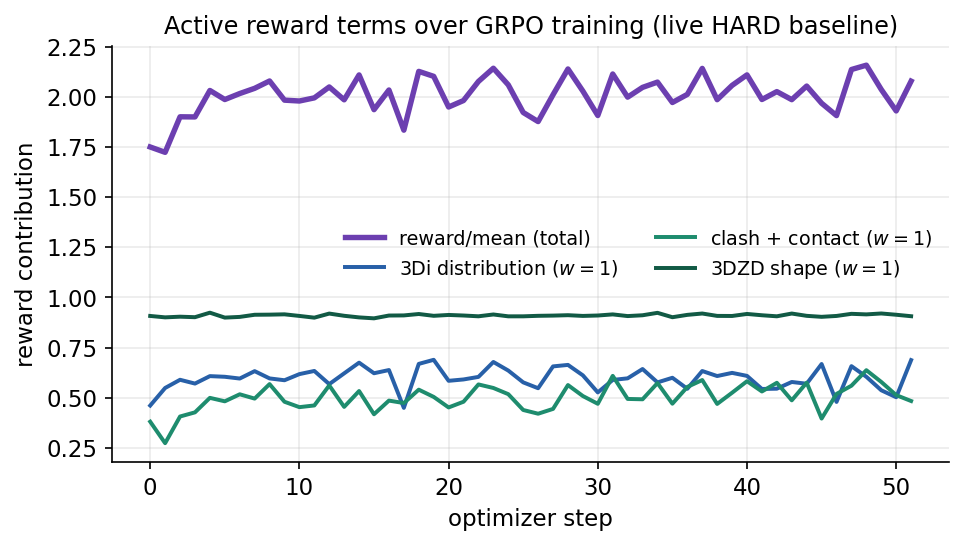
\includegraphics[width=0.92\linewidth]{figs/reward_terms.png}
\caption{Active reward terms over GRPO training (live HARD baseline,
\ttk{...chord\_nodist\_accum10\_seqtrack}). The total reward (\textcolor{lfLine}{purple})
rises from $1.75$ to $\sim\!2.08$; the 3DZD shape term sits near its ceiling ($\sim\!0.91$)
while the 3Di-distribution and clash+contact terms climb. CHORD SFT is a loss (not a reward
term) and is shown in Fig.~\ref{fig:diag}d.}
\label{fig:terms}
\end{figure}

\subsection{Distribution reward: 3Di interface-histogram alignment}
\label{sec:dist}
\ttk{w\_3di\_dist}$=1.0$. This was the first reward that realigned our interfaces. Build the 3Di
token histogram of a design as a blend of the whole-binder and interface-restricted histograms
($\beta_b=\ttk{dist\_binder\_frac}=0.5$), and reward closeness to a fixed reference histogram
computed from the Complexa-38 designs, under total-variation distance:
\[
h^{\mathrm{mix}}=(1-\beta_b)\,h^{I}_{\mathrm{3Di}}+\beta_b\,h^{\mathrm{bd}}_{\mathrm{3Di}},
\qquad
\R_{\mathrm{3Di}}=1-\TV\!\big(h^{\mathrm{mix}},\,h^{\mathrm{Complexa38}}_{\mathrm{3Di}}\big),
\quad
\TV(p,q)=\tfrac12\!\sum_k|p_k-q_k|,
\]
with an interface-collapse penalty $\R_{\mathrm{3Di}}\!\mathrel{+}=\ttk{dist\_iface\_penalty}=-1.0$
whenever $|I|<\ttk{dist\_min\_iface}=4$ (a design with almost no interface cannot game the
histogram). Offline this term is genuinely pass-predictive and \emph{shifts the distribution the
right way}: our D-heavy, monotonous interfaces move toward the V-rich, diverse Complexa profile,
reducing 3Di TV to the reference; the effect peaks around training step $\sim\!125$ before
diverging. Reference: \ttk{grpo\_dist\_reference\_complexa38\_binder.json}; the AA-distribution
twin (\ttk{w\_aa\_dist}) is tracked but kept off.

\emph{Evidence.} The offline TV study (Protenix-scored pools, $\sim\!3.7$k designs/arm)
shows the reward moves the 3Di distribution toward the Complexa reference, and only the 3Di
axis (its target) --- the AA axis, whose reward is off, does not improve:

\begin{table}[htbp]
\centering
{\renewcommand{\arraystretch}{1.2}%
\begin{tabular}{@{}>{\raggedright\arraybackslash}p{6.4cm}
                    >{\centering\arraybackslash}p{2.3cm}
                    >{\centering\arraybackslash}p{2.3cm}
                    >{\centering\arraybackslash}p{1.7cm}@{}}
\toprule
\textbf{TV to Complexa-38 ref}\ $\downarrow$ & \textbf{pre-GRPO} & \textbf{$+$3Di reward} & \textbf{$\Delta$}\\
\midrule
\rowcolor{dTint}3Di, interface           & $0.548$ & $0.413$ & $-0.135$\\
\rowcolor{dTint}3Di, whole binder        & $0.437$ & $0.299$ & $-0.138$\\
AA, interface \small(reward off)         & $0.414$ & $0.431$ & $+0.017$\\
\midrule
Protenix pass\,\% \small($\uparrow$, offline label) & $5.61$ & $2.97$ & $-2.64$\\
\bottomrule
\end{tabular}}
\caption{Offline distribution ablation on the Complexa-38 benchmark ($100$ designs/target,
target-balanced). Each TV cell is the total-variation distance between the arm's aggregate
interface (or whole-binder) histogram and the fixed Proteina-Complexa reference histogram
(\ttk{grpo\_dist\_reference\_complexa38\_binder.json}); lower is closer to native. Columns compare
the pre-GRPO policy against the $+$3Di-reward arm (\ttk{grpo\_aa2x\_s575\_a8}); $\Delta$ is the change. The reward drives only
the 3Di axis it targets (\textcolor{dLine}{blue} rows, $\approx\!-0.14$); the AA axis, whose reward is off, is
unchanged --- confirming the effect is causal, not a generic side-effect. The last row is the
Protenix pass rate (pTM$>\!0.80\wedge$ipTM$>\!0.70$, higher is better; offline label only, never a
reward): matching the interface 3Di distribution does \emph{not} by itself buy pass rate at this
checkpoint ($5.61\%\!\to\!2.97\%$), foreshadowing the sequence/structure/pass tension quantified in
Table~\ref{tab:seqablation}.}
\label{tab:distablation}
\end{table}
In-training the same shift appears live: \ttk{dist/tv\_3di} falls $0.585\!\to\!0.363$
(interface) and $0.480\!\to\!0.262$ (binder) over the first $52$ steps, while \ttk{dist/tv\_aa}
holds flat at $\sim\!0.40$ (Fig.~\ref{fig:diag}a).

\subsection{Geometry reward: smooth clash + interface contact}
\ttk{w\_clash\_contact}$=1.0$. Computed directly on the generated backbone (C$\alpha$ plus
C$\beta$, \ttk{clash\_include\_cb}). A soft-core clash energy penalizes atom pairs closer than
$d_c=\ttk{clash\_d\_clash}=2.2$\,\AA\ (soft width $\ttk{clash\_soft}=0.5$) across chains and for
non-local intra-binder pairs ($|i-j|>\ttk{clash\_seq\_sep}=2$); a triangular band rewards a
sensible interface-contact fraction $f$ (peak at $\ttk{frac\_peak}=0.16$, zero below
$\ttk{frac\_lo}=0.05$ and above $\ttk{frac\_hi}=0.4$, contact cutoff $\ttk{contact\_d0}=8$\,\AA):
\[
\R_{\mathrm{geom}}=\exp\!\big(-\eclash/\kappa\big)\cdot\mathrm{band}(f;\,0.05,0.16,0.4),
\qquad \kappa=\ttk{clash\_scale}=50 .
\]
This term is the guard that keeps the distribution reward honest: without it, the 3Di reward can
be gamed by interpenetrating the antigen (validated: $\eclash\!\to\!110$, interface fraction
$0.47$ vs native $0.12$--$0.15$). With it, interface fraction is pulled \emph{toward} native.
\emph{Evidence:} live, \ttk{clash/E\_clash} falls $36\!\to\!19$ while interface fraction stays
in the native band ($\approx\!0.18\text{--}0.28$) rather than blowing up (Fig.~\ref{fig:diag}c).
The ablation isolates the guard's effect on the interpenetration failure mode. As in \S\ref{sec:dist},
we score complete arms on the Complexa-38 benchmark ($100$ designs $\times\,38$ targets, target-balanced),
computing the exact geometry reward on every generated \ttk{\_complex.pdb} backbone:

\begin{table}[htbp]
\centering
{\renewcommand{\arraystretch}{1.2}%
\begin{tabular}{@{}>{\raggedright\arraybackslash}p{5.7cm}
                    >{\centering\arraybackslash}p{2.0cm}
                    >{\centering\arraybackslash}p{1.8cm}
                    >{\centering\arraybackslash}p{2.2cm}
                    >{\centering\arraybackslash}p{1.7cm}@{}}
\toprule
\textbf{Arm (Complexa-38)} & \textbf{$\eclash$ $\downarrow$} & \textbf{iface $f$} & \textbf{contact band $\uparrow$} & \textbf{pass\,\% $\uparrow$}\\
\midrule
LeFlur pre-GRPO base                                        & $24.7$  & $0.227$ & $0.61$ & $5.61$\\
$+$3Di reward                       & $118.8$ & $0.481$ & $0.06$ & $1.26$\\
\rowcolor{aTint}$+$3Di reward $+$ clash $+$ contact guard (\ttk{w\_clash\_contact}$=1$) & $\mathbf{11.1}$ & $\mathbf{0.194}$ & $\mathbf{0.70}$ & $\mathbf{4.82}$\\
passing Complexa (reference)                                & $1.7$   & $0.140$ & $0.51$ & $28.80$\\
\bottomrule
\end{tabular}}
\caption{Offline geometry ablation on the $38$-target Complexa benchmark ($100$ designs/target,
mean of per-target means). $\eclash$ = soft-core clash energy on the generated backbone
(C$\alpha$+C$\beta$, lower is better); iface $f$ = fraction of binder residues at the interface;
contact band = the $\mathrm{band}(f;0.05,0.16,0.40)$ reward term (higher is better); pass\,\% =
Protenix pass rate (pTM$>\!0.80\wedge$ipTM$>\!0.70$; offline label only, never a reward). Rows: the
pre-GRPO policy, the 3Di-distribution reward run \emph{without} the geometry guard, the same run
\emph{with} the guard (\textbf{adopted}, teal), and the passing-Complexa designs as a native-like
reference. \ttk{grpo3di\_s750\_a8} (no guard) vs \ttk{grpo\_multitgt\_s125\_a8} (with guard). The
guard not only restores native-like geometry but recovers most of the pass rate the unguarded
reward destroyed ($1.26\!\to\!4.82\%$).}
\label{tab:geomablation}
\end{table}
Without the guard the 3Di reward is gamed by driving the binder \emph{through} the antigen
($\eclash\!=\!118.8$, $f\!=\!0.481$), collapsing the contact band to $0.06$; adding the guard
cuts clash to $11.1$ and lifts the band to $0.70$ --- above the passing-Complexa reference ---
by pulling $f$ back to $0.19$, exactly where passing designs concentrate ($f\!\approx\!0.16$,
Fig.~\ref{fig:band}).

\begin{figure}[h]
\centering
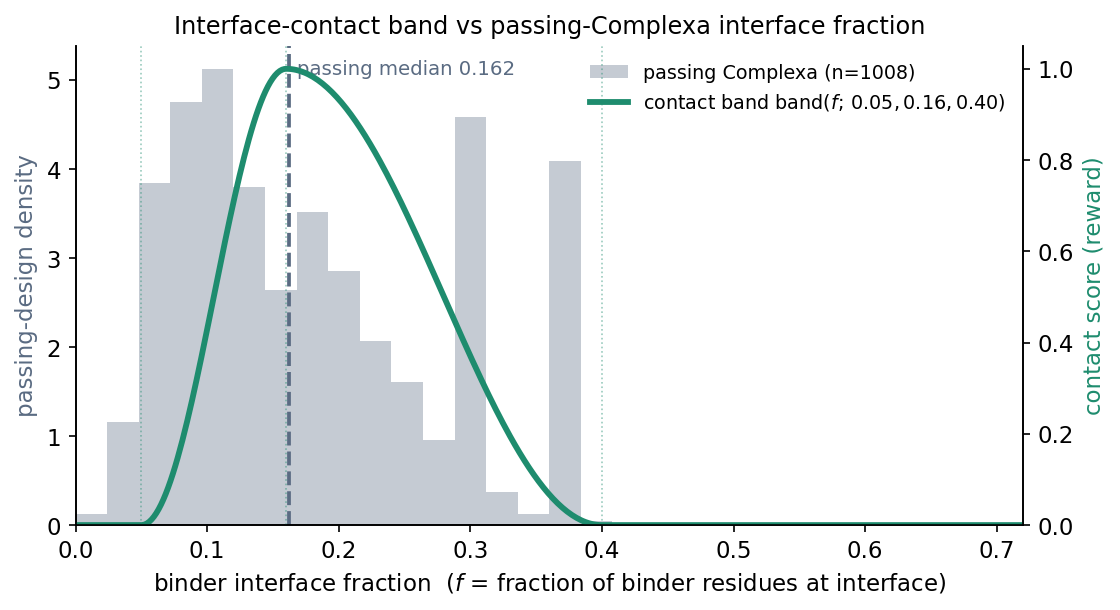
\includegraphics[width=0.86\linewidth]{figs/contact_band.png}
\caption{Interface-contact band $\mathrm{band}(f;0.05,0.16,0.40)$
(\textcolor{aLine}{teal}) overlaid on the interface-fraction distribution of the $1008$ passing
Complexa designs (\textcolor{ioLine}{gray}). The band peaks at the passing median
($f=0.162$) and is zero outside $[0.05,0.40]$, so the interpenetrating rollouts of the
unguarded arm ($f\!\approx\!0.47$) receive no contact reward.}
\label{fig:band}
\end{figure}

\subsection{MPNN-based reward: 3DZD interface shape complementarity}
\ttk{w\_shape}$=1.0$. Measured on the LigandMPNN-packed all-atom complex (\S2, pack branch).
For the interface patches of antigen and binder we compute crop-safe $\Delta$SASA patch
descriptors, expand each in 3D Zernike descriptors, and score complementarity as the raw Pearson
correlation of the two descriptor vectors:
\[
\R_{\SC}=\SC_{\mathrm{3DZD}}\!\big(\widehat Y^{I}_{\mathrm{ag}},\,\widehat Y^{I}_{\mathrm{bd}}\big).
\]
This is the reward that attacks the diagnosed shape limitation.

\emph{Discriminator (motivation).} On LigandMPNN-packed all-atom complexes, $\R_{\SC}$ is the
strongest Protenix-free pass/fail filter found (AUROC $0.73$): our designs score
$0.918\pm0.025$ against $0.956\pm0.008$ for passing Complexa designs --- a real $\approx\!0.04$
all-atom gap the reward is meant to close.

\emph{Ablation (offline).} As in \S\ref{sec:dist} and \S3.2 we score complete arms on the
Complexa-38 benchmark ($100$ designs $\times\,38$ targets, target-balanced), reporting \emph{both}
the Protenix- and pack-free \emph{backbone} proxy (raw-Pearson 3DZD SC on the generated
N/C$\alpha$/C interface patches, no side chains) \emph{and} the \emph{all-atom} $\R_{\SC}$ the
reward actually optimizes (LigandMPNN-packed full-atom complex, $3$ denoising steps $\times\,4$
samples), plus the Protenix pass rate (offline label):

\begin{table}[htbp]
\centering
{\renewcommand{\arraystretch}{1.2}%
\begin{tabular}{@{}>{\raggedright\arraybackslash}p{5.4cm}
                    >{\centering\arraybackslash}p{2.3cm}
                    >{\centering\arraybackslash}p{2.4cm}
                    >{\centering\arraybackslash}p{1.7cm}@{}}
\toprule
\textbf{Arm (Complexa-38)} & \textbf{backbone SC} $\uparrow$ & \textbf{all-atom SC} $\uparrow$ & \textbf{pass\%} $\uparrow$\\
\midrule
LeFlur pre-GRPO base                                        & $0.886\pm0.004$ & $0.906\pm0.004$ & $5.61$\\
$+$3Di reward $+$ geom guard (\ttk{grpo\_multitgt\_s125})   & $0.888\pm0.006$ & $0.915\pm0.004$ & $4.82$\\
\rowcolor{aTint}$+$3DZD shape reward (\ttk{grpo\_sc\_s125})  & $0.888\pm0.004$ & $0.911\pm0.004$ & $4.92$\\
passing Complexa (reference)                                & $0.886\pm0.009$ & $\mathbf{0.940\pm0.004}$ & $28.80$\\
\bottomrule
\end{tabular}}
\caption{Offline shape ablation on the $38$-target Complexa benchmark ($100$ designs/target, mean
of per-target means $\pm$ s.e.m.\ across the $38$ targets). \textbf{backbone SC} = raw-Pearson
3D-Zernike shape complementarity of crop-safe $\Delta$SASA interface patches on the generated
\emph{backbone} (N/C$\alpha$/C, no side chains); \textbf{all-atom SC} = the \emph{same} descriptor
on the LigandMPNN-packed full-atom complex ($3$ denoising steps $\times\,4$ samples) --- the
quantity $\R_{\SC}$ actually optimizes. \textbf{pass\%} $=$ Protenix pTM$>\!0.80\wedge$ipTM$>\!0.70$
(offline label only, never a reward). On the \emph{backbone} proxy all four arms are statistically
indistinguishable ($\approx\!0.887$) --- backbone shape complementarity is already saturated at the
native level. But on the \emph{all-atom} pack the discriminating gap appears: passing Complexa
scores $0.940$ against the pre-GRPO base's $0.906$ (the $\approx\!0.03$--$0.04$ AUROC-$0.73$ gap
this reward targets), and it is invisible to the backbone proxy. Every trained arm moves all-atom
SC toward Complexa in a paired per-target test --- the dedicated shape reward \ttk{grpo\_sc\_s125}
by $+0.005$ ($t\!=\!2.9$), \ttk{grpo\_multitgt\_s125} by $+0.009$ ($t\!=\!3.7$) --- but each closes
only a fraction of the $+0.034$ gap this early, and none is a pass-rate win.}
\label{tab:shapeablation}
\end{table}
The two SC columns are the point: LeFlur's \emph{backbone} interfaces already match passing
Complexa, so a backbone-only reward would be inert --- the shape deficit lives entirely in all-atom
packing, where a real $\approx\!0.03$--$0.04$ gap to the passing model ($0.906\!\to\!0.940$)
survives, which is exactly why $\R_{\SC}$ is scored on the LigandMPNN-packed all-atom complex. GRPO
with the shape reward moves the packed metric significantly in the right direction ($+0.005$ paired,
$t\!=\!2.9$) but closes only a fraction of that gap at step $125$; in training \ttk{shape/sc\_mean}
holds $\approx\!0.91$ on the packed complex (Fig.~\ref{fig:diag}b), just under the packed ceiling.
The all-atom SC-clash from the same pack (\ttk{w\_sc\_clash}) is tracked but kept out of the
gradient.

\subsection{Dense sequence reward: CHORD SFT distillation}
\ttk{sft\_mu}$=0.1$. The scalar AAR reward (agreement with the MPNN design) moved rollout AAR by
only $\sim\!+0.013$ and did not transfer --- a single scalar is a weak signal for a per-position
prediction problem. It is replaced by a \emph{dense} supervised term: a token-level
cross-entropy of the policy's own sequence-endpoint prediction toward the LigandMPNN-designed
binder sequence $a^{\ast}$ on the policy's \emph{own} backbone (DAgger: expert queried on the
learner's states). It is blended into GRPO as the CHORD convex objective (arXiv:2508.11408):
\[
\mathcal L=(1-\mu)\,\mathcal L_{\mathrm{GRPO}}+\mu\,\mathcal L_{\text{SFT-}\phi}+\beta\,\mathrm{KL},
\qquad \mu=0.1,\ \ \beta=0 .
\]
Let $p_{s,l}=\pi_\theta(a^{\ast}_l\mid x_{t_s})$ be the policy's probability of the expert token
at supervised step $s$, position $l$. The supervised mask and the detached CHORD weight are
\[
m_{s,l}=\underbrace{\mathrm{sup}_l}_{\text{binder}}\ \wedge\
        \mathrm{gen}^{\text{seq}}_l\ \wedge\
        \underbrace{[x^{\text{seq}}_{s,l}{=}\text{mask}]}_{\ttk{masked\_only}},
\qquad
\phi_{s,l}=p_{s,l}\,(1-p_{s,l})\ \ (\text{detached}),
\]
\[
\ell_s=\frac{\sum_l m_{s,l}\,\phi_{s,l}\,(-\log p_{s,l})}{\sum_l m_{s,l}\,\phi_{s,l}},
\qquad
\mathcal L_{\text{SFT-}\phi}=\frac1{|S|}\sum_{s\in S}\ell_s .
\]
$\phi$ peaks at $p{=}0.5$ and vanishes as $p\!\to\!0,1$: it zeroes the high-$p$ \emph{consensus}
tokens (the generic buried-hydrophobic core --- exactly the whole-binder failing mode that made
naive MPNN agreement anti-predictive, AUROC $0.29$) and the low-$p$ \emph{rejected} tokens (no
wholesale copying), so only genuinely contested positions carry gradient. This lets scope safely
widen to the whole binder (\ttk{sft\_scope=binder}): $\phi$ is a finer guard than an interface
mask and gives a far denser gradient. The HARD baseline uses \ttk{sft\_label=soft} (KL toward the
teacher's full per-position distribution); the per-token arm uses \ttk{sft\_label=hard} (CE toward
$a^{\ast}$) for a clean A/B. The gradient reaches the seq head because \ttk{sequence\_tokens} is
trainable; $\mu{=}0$ recovers pure GRPO.
\emph{Evidence:} live, \ttk{sft/ce\_loss} falls $2.04\!\to\!1.82$ (Fig.~\ref{fig:diag}d) while the
train-time rollout interface AAR (\ttk{aar/aar\_iface\_mean}, wandb --- unaffected by the offline chain
bug) rises only modestly ($0.126\!\to\!0.146$) over these first steps. Between-design novelty stays high
throughout --- but, as \S\ref{sec:seqcomplex} shows, that is \emph{not} evidence against collapse: the
novelty terms are blind to the per-design poly-alanine drift, which emerges later in training (by the
benchmark-sampler reading of step $325$) and is caught only by the per-design $\mathrm{LC}$ statistic and
the \ttk{dist/tv\_aa} distribution watch.

\emph{Ablation (offline, $100$ designs/target).} We score each arm through the cold A8 offline sampler
($\mathrm{nsteps}{=}200$, $T_{\mathrm{seq}}{=}0.273$, $\mathrm{stoch}_{\mathrm{seq}}{=}20$), generating
$100$ designs on each of the $38$ Complexa targets ($3800$ designs/arm), and on each generated backbone
query ProteinMPNN (\ttk{v\_48\_020}, antigen fixed) for \textbf{AAR} (fraction of binder positions where a
low-temperature redesign reproduces the generated residue --- agreement with the expert the SFT distils
toward) and $\mathbf{C_{\mathrm{mpnn}}}$ (teacher-forced likelihood of the generated sequence ---
seq$\leftrightarrow$struct consistency), at whole-binder and interface scope, against the pre-GRPO base
and the passing-Complexa ceiling (Table~\ref{tab:seqablation}). \emph{All AAR/$C_{\mathrm{mpnn}}$ numbers
here were recomputed after fixing a binder-chain identification bug in the offline scorer:} it had matched
the binder by chain \emph{letter}, but generation writes the antigen first (chain~A) and the binder second
(chain~B), so the scorer had been reporting ProteinMPNN self-recovery of the \emph{fixed native antigen}
rather than the designed binder --- collapsing every generated arm to $\approx\!0.17$ and masking all
between-arm spread. The corrected scorer sequence-matches the binder into the complex; it is a verified
no-op on the Complexa reference (where the binder is already chain~A, hence unchanged at $0.539$).
On the \emph{same} A8 gens we additionally score the Protenix pass rate (offline label only) and each of
the three structure-reward families introduced above --- whole-binder 3Di TV to the Complexa reference (\S3.1),
soft-core backbone clash energy $E_{\mathrm{clash}}$ (\S3.2), and all-atom 3DZD interface shape complementarity
(\S3.3), plus a chain-integrity diagnostic --- so a single table shows what the CHORD sequence objective does to every reward we have
presented (Table~\ref{tab:seqablation}).

\begin{table}[htbp]
\centering
\resizebox{\textwidth}{!}{%
{\renewcommand{\arraystretch}{1.2}%
\begin{tabular}{@{}>{\raggedright\arraybackslash}p{3.6cm}
                    >{\centering\arraybackslash}p{1.2cm}
                    >{\centering\arraybackslash}p{1.9cm}
                    >{\centering\arraybackslash}p{2.0cm}
                    >{\centering\arraybackslash}p{1.9cm}
                    >{\centering\arraybackslash}p{1.4cm}
                    >{\centering\arraybackslash}p{1.3cm}
                    >{\centering\arraybackslash}p{1.4cm}
                    >{\centering\arraybackslash}p{1.4cm}
                    >{\centering\arraybackslash}p{1.3cm}
                    >{\centering\arraybackslash}p{1.3cm}@{}}
\toprule
\textbf{Arm (Complexa-38)} & \textbf{pass\%} $\uparrow$ & \textbf{AAR} $\uparrow$ & \textbf{AAR iface} $\uparrow$ & $\mathbf{C_{\mathrm{mpnn}}}$ $\uparrow$ & $\mathbf{H}$ $\uparrow$ & \textbf{3Di TV} $\downarrow$ & $\mathbf{E_{\mathrm{clash}}}$ $\downarrow$ & \textbf{iface }$f$ $\to$nat & \textbf{SC} $\uparrow$ & \textbf{break\%} $\downarrow$\\
\midrule
LeFlur pre-GRPO base                                        & $5.61$ & $0.255\pm0.005$ & $0.222\pm0.004$ & $0.108\pm0.002$ & $3.61\pm0.02$ & $0.437$ & $24.7$ & $0.227\pm0.009$ & $0.906$ & $28.1$\\
$+$scalar AAR reward                                        & $4.32$ & $0.255\pm0.006$ & $0.229\pm0.006$ & $0.115\pm0.003$ & $\mathbf{3.26\pm0.04}$ & $\mathbf{0.348}$ & $11.5$ & $0.201\pm0.008$ & $\mathbf{0.920}$ & $\mathbf{18.0}$\\
\rowcolor{aTint}$+$CHORD SFT (\ttk{expertctx}), step $175$  & $2.92$ & $\mathbf{0.383\pm0.006}$ & $\mathbf{0.303\pm0.006}$ & $\mathbf{0.178\pm0.003}$ & $2.34\pm0.03$ & $0.412$ & $\mathbf{6.4}$ & $\mathbf{0.144\pm0.005}$ & $0.914$ & $18.8$\\
passing Complexa (reference)                                & $28.8$ & $0.539\pm0.008$ & $0.511\pm0.009$ & $0.273\pm0.007$ & $3.71\pm0.03$ & $0.253$ & $1.7$ & $0.140\pm0.012$ & $0.940$ & $0.5$\\
\bottomrule
\end{tabular}}}
\caption{\emph{Corrected 100-designs/target sweep} (chain-fixed offline scorer), reporting
\emph{every} reward family presented above (\S3.1--\S3.3) on the \emph{same} cold A8 gens as the
sequence metrics. Each arm: $100$ designs on each of $38$ Complexa targets ($3800$ designs/arm), cold A8
sampler ($\mathrm{nsteps}{=}200$, $T_{\mathrm{seq}}{=}0.273$, $\mathrm{stoch}_{\mathrm{seq}}{=}20$).
\textbf{pass\%} $=$ Protenix pTM$>\!0.80\wedge$ipTM$>\!0.70$ (offline label only, never a reward).
\textbf{AAR}/\textbf{AAR iface}/$\mathbf{C_{\mathrm{mpnn}}}$ $=$ ProteinMPNN redesign agreement and
consistency likelihood (\ttk{v\_48\_020}, $K{=}5$ draws, $T{=}0.1$; interface $=$ binder C$\alpha$ within
$8$\,\AA{} of any antigen C$\alpha$), target-balanced macro-means $\pm$ s.e.m.\ over targets.
$\mathbf{H}$ $=$ mean per-design Shannon entropy of the binder amino-acid composition
(bits, $\max=\log_2 20\approx4.32$; the collapse statistic of \S\ref{sec:seqcomplex}),
target-balanced macro-mean $\pm$ s.e.m.\ over targets --- higher $=$ more diverse, with the
passing-Complexa band ($\approx\!3.7$) as the healthy reference; the CHORD arm's drop to $2.34$ is
the poly-alanine collapse the \S\ref{sec:seqcomplex} guardrail targets.
\textbf{3Di TV} $=$ \emph{whole-binder} 3Di histogram TV distance to the Complexa reference (\S3.1,
lower $=$ closer; s.e.m.\ $\approx0.004$); $\mathbf{E_{\mathrm{clash}}}$ $=$ soft-core backbone interface
clash energy (\S3.2, lower $=$ fewer clashes); \textbf{iface }$f$ $=$ interface-contact fraction (\S3.2,
the quantity the contact band scores; $\to$nat $=$ closer to the passing/native band $f\!\approx\!0.14$--$0.16$
is better, \emph{not} monotone --- both over- and under-contacting hurt); \textbf{SC} $=$ \emph{all-atom} (LigandMPNN-packed) 3DZD
interface shape complementarity (\S3.3, the packed quantity $\R_{\SC}$ optimizes; s.e.m.\ $\approx0.004$);
\textbf{break\%} $=$ fraction of designs with $\ge\!1$ backbone C--N bond $>\!2$\,\AA{} (chain-integrity
diagnostic, lower $=$ better). Bold $=$ best \emph{trained} arm per column. All rows read through the
identical cold A8 sampler (directly comparable); interface-AAR deltas vs.\ base are given in the text.
\emph{The sequence and structure rewards move in opposite directions.} Dense CHORD SFT (\ttk{expertctx})
is the sole family that materially lifts AAR/$C_{\mathrm{mpnn}}$ and it also sharply de-clashes the
backbone ($E_{\mathrm{clash}}$ $24.7\!\to\!6.4$), pulls the interface-contact fraction from an
over-contacting $0.227$ onto the passing band ($f\!=\!0.144$, matching Complexa's $0.140$), and roughly
halves broken chains ($28.1\%\!\to\!18.8\%$),
yet the Protenix pass rate \emph{falls} ($5.61\%\!\to\!2.92\%$) and the whole-binder 3Di distribution
moves only partway toward Complexa ($0.437\!\to\!0.412$, vs.\ the Complexa floor $0.253$). The discarded
scalar AAR reward is $\approx$neutral on sequence ($+0.007$ interface) yet incidentally the strongest on
the structure diagnostics --- closest 3Di distribution ($0.348$), highest all-atom SC ($0.920$), fewest
breaks ($18.0\%$) --- while de-clashing ($24.7\!\to\!11.5$). All-atom SC now \emph{does} separate the
arms (base $0.906$ vs.\ Complexa $0.940$; every trained arm lifts it in a paired test), a gap the
backbone proxy of Table~\ref{tab:shapeablation} hid.}
\label{tab:seqablation}
\end{table}

\textbf{Dense CHORD SFT is the sole arm that materially lifts sequence agreement.} The featured CHORD
arm is the expert-context run (\ttk{expertctx}, step $175$): conditioning the SFT forward on the
\emph{expert's own} sequence context (rather than the policy's revealed tokens) raises interface AAR
$0.222\!\to\!0.303$ ($+0.081$) and whole-binder AAR $0.255\!\to\!0.383$ ($+0.128$), with
$C_{\mathrm{mpnn}}$ $0.108\!\to\!0.178$ --- a clear gain over the earlier policy-context formulation of
the same distillation, both read through the same cold A8 sampler. The whole-binder gain \emph{exceeds}
the interface gain and $C_{\mathrm{mpnn}}$ climbs alongside it, so this is a broad improvement in
seq$\leftrightarrow$struct coherence, not the narrow contested-position-only effect the $\phi$ guard was
expected to produce. The discarded \emph{scalar} AAR reward is by contrast $\approx$neutral ($+0.007$
interface, $+0.007$ $C_{\mathrm{mpnn}}$): a single scalar is too weak a signal for a per-position target
--- the motivation for the dense term. The gap to the Complexa ceiling ($0.511$ interface) remains
large, as expected this early in training.

\textbf{The structure rewards tell a partly opposite story --- a sequence/pass trade-off.}
Reading the same A8 gens through the three structure-reward families (\S3.1--\S3.3) exposes what the AAR
columns hide. The good news for CHORD is geometry: the featured \ttk{expertctx} arm sharply de-clashes the
backbone, dropping interface $E_{\mathrm{clash}}$ $24.7\!\to\!6.4$ (\S3.2) --- the lowest of any trained
arm, closest to the Complexa floor ($1.7$) --- with the neutral scalar-AAR arm at $11.5$, and it roughly
halves broken chains ($28.1\%\!\to\!18.8\%$). But the Protenix \textbf{pass rate falls as AAR rises}:
base $5.61\%\to$ scalar-AAR $4.32\%\to$ \ttk{expertctx} $2.92\%$ --- at this checkpoint the
sequence-recovery objective pulls the policy \emph{away} from foldable/dockable designs, not toward them
(pass is an offline label here, never a reward). The distribution and packing rewards favor the
\emph{scalar}-AAR arm: it moves the whole-binder 3Di histogram farthest toward Complexa (3Di TV
$0.437\!\to\!0.348$, floor $0.253$), packs the highest all-atom SC ($0.920$), and breaks the fewest chains
($18.0\%$), whereas \ttk{expertctx} --- the AAR leader --- moves the 3Di distribution only partway
($0.412$), i.e.\ it maximizes per-position agreement without fully matching the reference's interface
\emph{shape} vocabulary. Unlike the saturated backbone proxy of Table~\ref{tab:shapeablation}, all-atom SC
\emph{does} lift under GRPO (base $0.906\!\to\!0.914$--$0.920$ across trained arms; Complexa $0.940$). Net:
dense CHORD SFT buys sequence coherence, cleaner backbones, and more intact chains at a real cost in
Protenix pass; that tension is the central open question for this reward set.

\textbf{On the per-token clash combination.} We no longer list the per-token clash $+$ CHORD arm as a
separate row: the featured \ttk{expertctx} run \emph{has} the per-token clash reward active
(\ttk{per\_token\_clash} on, $\ttk{sft\_mu}{=}0.1$), so its interface $E_{\mathrm{clash}}$ of $6.4$ --- the
lowest of any trained arm --- \emph{is} that dense per-token structure advantage (\S3.5) at work, now
carried by the $E_{\mathrm{clash}}$ column above rather than by a standalone line. An earlier
policy-context checkpoint of this blend had sat below base on AAR under matched A8 sampling, reading as the
structure signal fighting the sequence signal; the expert-context formulation removes that conflict ---
\ttk{expertctx} is now simultaneously the AAR leader and the least-clashing arm --- so per-token structure
credit and CHORD sequence distillation are compatible, not antagonistic. The residual open item is the
pass-rate cost documented above.

\textbf{The cold A8 sampler and the training-rollout sampler are not interchangeable.} Every number in
Table~\ref{tab:seqablation} is read through the cold A8 sampler ($\mathrm{nsteps}{=}200$,
$T_{\mathrm{seq}}{=}0.273$, $\mathrm{stoch}_{\mathrm{seq}}{=}20$), whereas the policy is \emph{trained}
under a much hotter, shorter rollout ($\mathrm{nsteps}{=}40$, $T_{\mathrm{seq}}{=}1.0$,
$\mathrm{stoch}_{\mathrm{seq}}{=}1$). Reading one expert-context CHORD checkpoint
(\ttk{grpo\_expertctx\_cont50\_step175}, the featured CHORD example in Table~\ref{tab:seqablation})
through \emph{both} samplers --- $3800$ designs each, identical weights --- shows the gap is large and
one-sided (Table~\ref{tab:sampler}; its A8 row is exactly the \ttk{expertctx} row of
Table~\ref{tab:seqablation}): the cold A8 sampler lifts
whole-binder AAR $0.270\!\to\!0.383$ ($+0.113$), interface AAR $0.223\!\to\!0.303$ ($+0.080$),
$C_{\mathrm{mpnn}}$ $0.097\!\to\!0.178$, and the Protenix pass rate $1.61\%\!\to\!2.92\%$
(pTM $0.626\!\to\!0.646$, ipTM $0.330\!\to\!0.336$). So the ablation table measures the
\emph{policy $+$ cold sampler} jointly, and a checkpoint's training-rollout numbers understate what the
same weights can produce; the between-arm comparisons in Table~\ref{tab:seqablation} are fair
\emph{relative} readings (all arms share the A8 sampler), but any single arm's absolute pass/AAR
depends on the sampler as much as on the weights.

\begin{table}[htbp]
\centering
{\renewcommand{\arraystretch}{1.2}%
\begin{tabular}{@{}>{\raggedright\arraybackslash}p{6.0cm}
                    >{\centering\arraybackslash}p{1.5cm}
                    >{\centering\arraybackslash}p{2.0cm}
                    >{\centering\arraybackslash}p{2.2cm}
                    >{\centering\arraybackslash}p{1.7cm}@{}}
\toprule
\textbf{Sampler (same ckpt, \ttk{expertctx} step $175$)} & \textbf{pass} $\uparrow$ & \textbf{AAR} $\uparrow$ & \textbf{AAR iface} $\uparrow$ & $\mathbf{C_{\mathrm{mpnn}}}$ $\uparrow$\\
\midrule
\rowcolor{aTint}benchmark (div.\ penalty on)                    & $\mathbf{3.11\%}$ & $\mathbf{0.385\pm0.001}$ & $\mathbf{0.307\pm0.002}$ & $0.154$\\
cold A8 ($200$ steps, $T{=}0.273$, stoch $20$)                & $2.92\%$ & $0.383\pm0.006$ & $0.303\pm0.006$ & $\mathbf{0.178}$\\
training rollout ($40$ steps, $T{=}1.0$, stoch $1$)           & $1.61\%$ & $0.270\pm0.005$ & $0.223\pm0.003$ & $0.097$\\
\bottomrule
\end{tabular}}
\caption{\emph{Sampler dependence on identical weights.} One expert-context CHORD checkpoint
(\ttk{grpo\_expertctx\_cont50\_step175}), $100$ designs on each of $38$ Complexa targets ($3800$
designs) under each sampler, same offline scorers as Table~\ref{tab:seqablation}. \textbf{pass} $=$
Protenix pTM$>\!0.80\ \wedge\ $ipTM$>\!0.70$; AAR/$C_{\mathrm{mpnn}}$ as in Table~\ref{tab:seqablation}.
Three samplers on \emph{identical weights}: the benchmark sampler (diversity penalty on, the
configuration used for all main-table pass rates) and the cold A8 sampler both beat the training
rollout across the board ($+0.11$ whole-binder AAR, pass $\sim\!1.9\times$); benchmark and cold A8
are within noise on AAR/pass while the rollout trails badly. So all offline-scored ablations read
the \emph{policy $+$ sampler} jointly and understate the training-rollout checkpoint; conversely
$C_{\mathrm{mpnn}}$ is highest under cold A8, i.e.\ the lower-temperature stochastic sampler yields
the most MPNN-self-consistent sequences.}
\label{tab:sampler}
\end{table}

\emph{End-to-end (Protenix-refolded, step 50).} Folding the full live arm at training step $50$ on
Complexa-38 ($100$ designs $\times\,38=3800$ designs, Protenix-scored) gives a $\mathbf{3.7\%}$ pass rate
($139/3800$; pass $=$ pTM$>\!0.80\ \wedge\ $ipTM$>\!0.70$) over $\mathbf{32/38}$ targets --- broad
coverage. Aligning each Protenix refold back onto the generated complex exposes a fold/dock split: the
binder \emph{monomer} fold is reproduced (binder-only C$\alpha$-RMSD median $2.4$\,\AA), yet the docking
\emph{pose} disagrees (antigen-aligned binder L-RMSD median $29.5$\,\AA) --- the high ipTM is Protenix's
confidence in \emph{an} interface, not the generated one. \textbf{Net:} the binder fold is generated well,
but Protenix re-docks it --- \emph{docking-pose fidelity} (dock-as-generated), not fold quality, is the
clearest open lever at this checkpoint. The CHORD-SFT sequence lift (Table~\ref{tab:seqablation}) is
realized by the expert-context per-token run (\ttk{expertctx}, which carries this same per-token clash
reward); the residual gap is the pass-rate cost that accompanies the AAR lift, not a failure of the SFT
term to express under matched scoring.

\subsection{Sequence anti-degeneracy: a linguistic-complexity floor and within-group Hamming diversity}
\label{sec:seqcomplex}
\ttk{w\_seq\_complexity}$=\lambda$ and \ttk{w\_seq\_hamming}$=w_h$ (both wired; off by default,
$\lambda{=}w_h{=}0$, so the reward is byte-identical to the runs above until either is turned on).

\textbf{The failure it guards against.} The CHORD arm \emph{learns then drifts}: read through the
benchmark sampler, the \ttk{expertctx} run peaks near step $175$ and degrades by step $325$ (pass
$3.11\%\!\to\!1.01\%$). The sequence-level cause is a \emph{poly-alanine mode collapse} --- extracting
the one-letter binder sequences at both checkpoints, alanine rises $13.3\%\!\to\!53.1\%$ (of all binder
residues), the mean per-design Shannon entropy falls $2.61\!\to\!1.85$ bits, and the fraction of designs
in which a single residue exceeds half the chain jumps $0.2\%\!\to\!36.7\%$ (many literal homopolymers,
top tripeptide \ttk{AAA}). This is textbook reward-hacking: poly-Ala is ProteinMPNN's safe
high-marginal-likelihood residue, so $C_{\mathrm{mpnn}}$ \emph{rises} against pass ($0.154\!\to\!0.178$,
anti-predictive) even as AAR --- MPNN's \emph{argmax} redesign, which never returns poly-Ala for a real
backbone --- \emph{falls} with pass ($0.386\!\to\!0.328$). The $\phi=p(1{-}p)$ guard of \S3.4 does not
catch it: $\phi$ zeroes \emph{consensus} positions, but a low-complexity sequence is precisely one whose
positions are high-confidence, so the collapse hides in the zeroed part of the CHORD gradient. The
within-group $k$-mer novelty (the existing $\nu^{\mathrm{aa}}/\nu^{\mathrm{3Di}}$ reward terms defined
below --- and in any case weight-$0$, so logged-only, throughout the CHORD runs) does not catch it
either: a group of \emph{diverse} degenerate modes (poly-A, poly-L, poly-S) scores high pairwise
novelty --- indeed \ttk{diversity/seq\_novelty\_mean} held $\approx\!0.91$ across the entire CHORD run
even as alanine climbed past half the chain. What discriminates both single-residue and
distributed collapse is a per-design \emph{complexity} statistic, with an \emph{absolute} floor
(calibrated to the healthy-reference band) rather than a relative one.

\textbf{Per-design complexity statistic.} We measure per-design collapse not with
composition entropy but with a \emph{linguistic-complexity} statistic read off the decoded string at low
$k$-mer order, where the separation actually lives. Extending the Table~\ref{tab:seqablation} entropy $H$ to hard $k$-mers over
all four rows (base, $+$scalar AAR, collapsed CHORD \ttk{expertctx}, passing Complexa; $k{=}1$--$7$)
shows that \emph{entropy} separates the rows best at $k{=}1$ and degrades monotonically with $k$
($\eta^2\,0.66\!\to\!0.04$), saturating toward $\log_2 W$ because $20^k\!\gg\!W$ makes almost every
high-order $k$-mer unique in \emph{every} design; whereas the \emph{coverage} (distinct-$k$-mer
fraction) separates best at $k{=}2$--$3$ ($\eta^2\,0.63/0.60$ vs.\ $0.30$ at $k{=}1$). The reason is
that $k{=}1$ entropy is blind to \emph{composition-preserving} repeats --- a sequence that reuses the
same amino-acid budget in a repetitive motif keeps $H$ high but collides at $k{=}2,3$ --- the exact
mode a coverage statistic catches.

For design $i$ with binder sequence $a_i$ of length $L_i$, let $W^{(k)}_i=L_i-k+1$ be the number of
overlapping $k$-mers and $u^{(k)}_i$ the number of \emph{distinct} ones. The order-$k$ coverage and the
linguistic complexity are
\[
\mathrm{cov}^{(k)}_i=\frac{u^{(k)}_i}{\min(20^k,\,W^{(k)}_i)}\in[0,1],
\qquad
\mathrm{LC}_i=\prod_{k=1}^{3}\mathrm{cov}^{(k)}_i\ \in[0,1].
\]
The product is a conjunction across orders: a deficit at \emph{any} $k$ multiplies the score down, so
$\mathrm{LC}_i$ is small for single-residue collapse (kills $\mathrm{cov}^{(1)}$), for distributed
few-residue mush (kills $\mathrm{cov}^{(1)},\mathrm{cov}^{(2)}$), and for composition-preserving repeats
(kills $\mathrm{cov}^{(2)},\mathrm{cov}^{(3)}$ while $\mathrm{cov}^{(1)}$ stays high) alike; truncating at
$k{=}3$ drops the saturated high-order factors ($\approx1$ for every design) that only add noise.
Measured on the Table~\ref{tab:seqablation} pools it is the single most discriminative aggregate we
found (Table~\ref{tab:diversitymetrics}): macro-mean $\mathrm{LC}$ is $0.519$ (base), $0.390$ ($+$scalar
AAR), $0.098$ (collapsed CHORD), and $0.574$ (passing Complexa) --- $\eta^2{=}0.63$ with a
collapsed-vs-Complexa Cohen's $d{=}5.84$,
against $d{=}4.1$ for the best single order ($k{=}2$ coverage) and $d{=}3.1$ for $k{=}1$ entropy. Like
$H$ it is a pure string statistic on the decoded binder (\ttk{\_decode\_binder\_seqs}), computed exactly
like the existing diversity signal, so no oracle, Protenix, or repack call is added. $\mathrm{LC}_i$ is
both the primary reward-side pressure against collapse --- an absolute per-design floor
(\S\ref{sec:seqcomplex}, ``the $\mathrm{LC}$ floor penalty'') --- and an always-on tracking diagnostic;
the \emph{between-design} Hamming term developed next is a complementary, mean-centered guard.

\textbf{The diversity reward.} Within a GRPO group every design targets the \emph{same} epitope at the
\emph{same} binder length --- the trainer draws one length per group and holds it fixed across all $G$
rollouts (\ttk{binder\_length\_min/max}, else the target's \ttk{spec.binder\_length}) --- so a group is a
set of $G$ equal-length strings and the position-wise Hamming distance between any two is well-defined.
For designs $i,j$ with binder sequences $a_i,a_j$ of common length $L$, the per-design within-group
diversity is the mean \emph{normalized} Hamming distance to the rest of the group,
\[
h_i=\frac1{G-1}\sum_{j\ne i}\frac1{L}\sum_{l=1}^{L}\mathbb 1\!\left[a_{i,l}\ne a_{j,l}\right]\ \in[0,1],
\]
so $h_i{=}0$ when design $i$ is a verbatim copy of the group and $h_i{=}1$ when it differs from every peer
at every aligned position. It is a pure string statistic --- a Hamming sibling of the existing
\ttk{jaccard\_novelty\_group}, singleton group $\mapsto 1$ --- so no oracle, Protenix, or repack call is
added.

\textbf{Hamming vs.\ the existing $k$-mer novelty.} The existing diversity terms $\nu^{\mathrm{aa}}_i$ and
$\nu^{\mathrm{3Di}}_i$ (the trainer's \ttk{jaccard\_novelty\_group}, weights
\ttk{w\_seq\_diversity}/\ttk{w\_struct\_diversity} --- both $0$ in every run to date, so tracked but never
graded) are mean pairwise $k$-mer-Jaccard \emph{set} distances ---
alignment-free and length-robust, but order-blind: they compare \emph{vocabularies}, not
\emph{positions}. Hamming is their positional complement, firing precisely on \emph{consensus
convergence} --- the group agreeing residue-by-residue toward one sequence --- which a shared-vocabulary
Jaccard can under-report. The equal-length group makes the position-wise metric available and cheap; we
add it as a sibling term, applied independently to the AA sequence and (optionally) the 3Di
structural-token string. Both metrics are \emph{between}-design: a group of individually degenerate but
mutually \emph{different} modes (poly-A, poly-L, poly-S) still scores high on both --- the per-design
internal-degeneracy failure remains the job of the $\mathrm{LC}$ floor, not of any pairwise term.

\textbf{What each metric actually captures.} Table~\ref{tab:diversitymetrics} measures all three
metrics on the four Table~\ref{tab:seqablation} pools and settles the division of labour. The
within-sequence $\overline{\mathrm{LC}}$ craters on the collapsed CHORD arm ($0.519\!\to\!0.098$) and is
\emph{highest} on passing Complexa ($0.574$): it is both the sharpest collapse detector
($\eta^2{=}0.63$) and \emph{success-aligned} (Complexa vs.\ collapsed Cohen's $d{=}{+}5.84$). The two
\emph{between}-design metrics behave oppositely. They barely register the collapse --- the collapsed arm
keeps $\bar h{=}0.766$ and $\bar\nu^{\mathrm{aa}}{=}0.782$, because its designs collapse to
\emph{different} degenerate modes and so stay mutually distant --- and, decisively, passing Complexa
scores the \emph{lowest} of any row on both ($\bar h{=}0.641$, $\bar\nu{=}0.624$; $d{=}{-}1.61$ and
$-1.83$ vs.\ collapsed). Good binders for a shared epitope \emph{converge}, so between-design diversity
is anti-aligned with pass \emph{at the population level}: maximizing $\bar h$ as an absolute objective
would push the policy \emph{away} from the passing distribution. This is exactly why the two terms play
different roles below --- $\mathrm{LC}_i$ as an absolute per-design floor (the collapse detector and
success signal), and $h_i$ only as a \emph{group-mean-centered} anti-consensus guard (\S\ref{sec:seqcomplex},
``group-normalization caveat''), never a maximization target.

\begin{table}[htbp]
\centering
\small
\begin{tabular}{lccc}
\toprule
 & \textbf{within-sequence} & \multicolumn{2}{c}{\textbf{between-design}} \\
\cmidrule(lr){2-2}\cmidrule(lr){3-4}
row & $\overline{\mathrm{LC}}$ & $\bar h$ (Hamming) & $\bar\nu^{\mathrm{aa}}$ (Jaccard) \\
\midrule
base                                    & $0.519\pm0.015$          & $0.896\pm0.003$ & $0.954\pm0.003$ \\
$+$scalar AAR                           & $0.390\pm0.019$          & $0.864\pm0.005$ & $0.927\pm0.004$ \\
collapsed CHORD (\ttk{expertctx}\,s175) & $\mathbf{0.098\pm0.006}$ & $0.766\pm0.005$ & $0.782\pm0.006$ \\
passing Complexa                        & $\mathbf{0.574\pm0.022}$ & $0.641\pm0.067$ & $0.624\pm0.075$ \\
\midrule
$\eta^2$ (row separation)               & $0.63$  & $0.42$  & $0.53$  \\
Cohen's $d$ (Complexa $-$ collapsed)    & $+5.84$ & $-1.61$ & $-1.83$ \\
\bottomrule
\end{tabular}
\caption{\textbf{The two new diversity metrics vs.\ the CHORD poly-alanine collapse}, on the same cold
A8 pools as Table~\ref{tab:seqablation} (base/AAR/collapsed $=3800$ designs each, $2274$ in multi-design
equal-length groups; passing Complexa $=1008$, $518$ grouped; $38$ Complexa targets; target-balanced
macro-mean $\pm$ s.e.m.). \emph{Within-sequence} $\overline{\mathrm{LC}}{=}\prod_{k=1}^{3}\mathrm{cov}^{(k)}$
fires on the collapse ($0.098$) and ranks passing Complexa highest ($0.574$): a per-design detector that
is also success-aligned. The \emph{between-design} metrics --- group pairwise Hamming $\bar h$ and the
incumbent $k$-mer-Jaccard novelty $\bar\nu^{\mathrm{aa}}$ (\ttk{w\_seq\_diversity}) --- are nearly blind
to the collapse (the collapsed arm stays $\approx\!0.77$--$0.78$) and are \emph{anti}-aligned with pass
(Complexa scores lowest, negative $d$). Hence $\mathrm{LC}$ is wired as the per-design floor and $h$ as a
mean-centered within-group guard, not an absolute objective. Computed by
\ttk{scripts/\_diversity\_metrics\_table.py}.}
\label{tab:diversitymetrics}
\end{table}

\textbf{Folding into the reward.} The two new anti-degeneracy signals enter alongside the two $k$-mer
novelties (\ttk{\_compute\_rewards}) --- a positive between-design Hamming reward $+w_h h_i$ and a negative
per-design complexity floor $-\lambda g_i$:
\[
R_i=\underbrace{c_i}_{\text{conf}}+\underbrace{s_i}_{\text{struct}}
   +w_{\mathrm{sd}}\,\nu^{\mathrm{aa}}_i+w_{\mathrm{td}}\,\nu^{\mathrm{3Di}}_i
   \;+\;w_{h}\,h_i\;-\;\lambda\,g_i,
\]
with $w_h=\ttk{w\_seq\_hamming}\ge0$ the between-design Hamming weight and $\lambda=\ttk{w\_seq\_complexity}\ge0$
the per-design complexity-floor weight, whose penalty $g_i$ is defined below. Both feed the same
group-relative advantage $A_i=(R_i-\bar R)/(\sigma_R+\varepsilon)$ (GRPO) or $A_i=R_i-\bar R$ (Dr.\ GRPO)
and the unchanged CHORD objective of \S3.4. For the Hamming term, a design more different from its peers
than the group average earns positive advantage --- its trajectory log-prob is pushed \emph{up} --- while
a near-duplicate is pushed \emph{down}, spreading the group apart directly.

\textbf{The group-normalization caveat.} Because both advantage variants mean-center, the diversity
reward enters the gradient only through its \emph{within-group variation},
\[
+w_h\,h_i\ \longrightarrow\ +w_h\,(h_i-\bar h)\quad\text{in }A_i .
\]
While the group is \emph{mixed} --- a collapsing consensus plus a few outliers --- $h_i-\bar h\neq0$, the
outliers are rewarded and the consensus suppressed, and the group re-spreads. If a group has
\emph{already} collapsed to one sequence ($h_i\!\approx\!0\ \forall i$) then $h_i-\bar h\!\approx\!0$ and
the term vanishes under normalization; like every within-group diversity signal it prevents collapse but
cannot rescue a group that is wholly gone. This is why $\bar h$ and $\overline{\mathrm{LC}}$ are
\emph{tracked} every step (below), so the diversity weight can be raised while groups are still mixed.

\textbf{The $\mathrm{LC}$ floor penalty.} The between-design Hamming term above cannot see per-design
internal degeneracy (Table~\ref{tab:diversitymetrics}: the collapsed arm keeps $\bar h{=}0.766$), and a
pure diversity \emph{bonus} would fight the (converging, non-uniform) passing-Complexa distribution. The
primary anti-collapse pressure is therefore a \emph{per-design}, absolute floor on $\mathrm{LC}_i$,
penalized as $-\lambda g_i$ with $\lambda=\ttk{w\_seq\_complexity}\ge0$ --- exactly the statistic that both
craters on the collapse and ranks passing Complexa highest.

\textbf{Absolute-floor penalty.} $\mathrm{LC}_i$ is turned into a one-sided soft hinge that is
\emph{identically zero inside the healthy band} and ramps to $1$ at full collapse --- a two-threshold
linear ramp with edges calibrated from the measured rows (healthy references
$\mathrm{LC}\!\approx\!0.52$--$0.57$; full poly-Ala collapse $\mathrm{LC}\!\approx\!0.10$):
\[
g_i=\mathrm{clip}\!\left(\frac{\mathrm{LC}_{\mathrm{hi}}-\mathrm{LC}_i}{\mathrm{LC}_{\mathrm{hi}}-\mathrm{LC}_{\mathrm{lo}}},\,0,\,1\right)\ \in[0,1]
\qquad (\mathrm{LC}_{\mathrm{hi}}{=}0.45,\ \mathrm{LC}_{\mathrm{lo}}{=}0.15).
\]
A \emph{single} floor now covers both the single-residue and the distributed/repeat modes that
previously needed a separate entropy hinge and dominant-fraction ceiling combined by an \textsc{or}, so
$g_i=0$ for every healthy design (base and passing Complexa both sit above $\mathrm{LC}_{\mathrm{hi}}$)
and $g_i\!\to\!1$ for a homopolymer (Fig.~\ref{fig:lcfloor}). Because it is clamped to zero in the band, the term exerts \emph{no
force on the healthy distribution} --- it is a guardrail, not a pressure that reshapes normal designs,
unlike a diversity \emph{bonus}.

\begin{figure}[htbp]
\centering
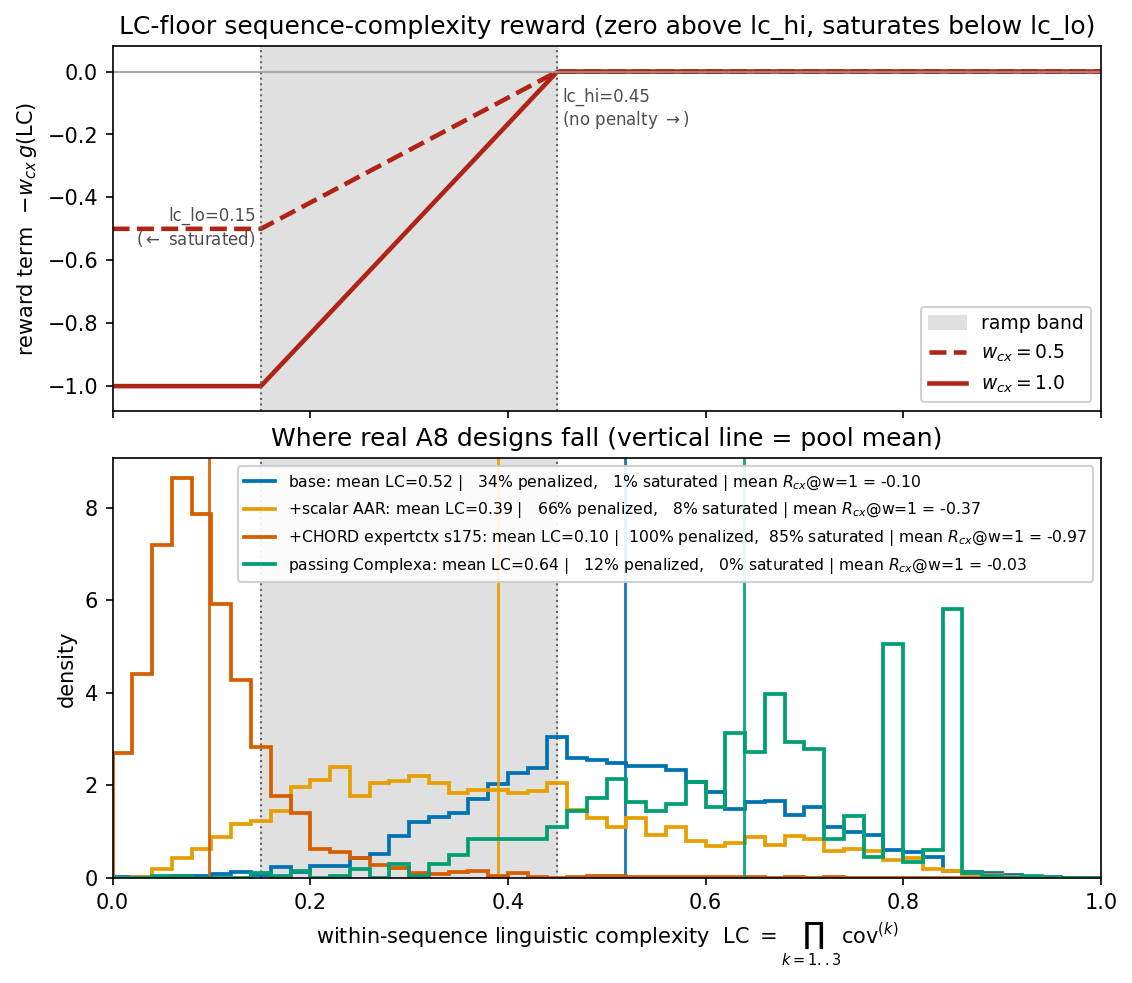
\includegraphics[width=0.92\linewidth]{figs/lc_floor_reward.png}
\caption{The $\mathrm{LC}$-floor sequence-complexity reward, calibrated against real designs.
\textbf{(top)} the reward term $-\lambda\,g_i$ as a function of $\mathrm{LC}_i$ for
$\lambda{=}\ttk{w\_seq\_complexity}\in\{0.5,1.0\}$: identically zero above
$\mathrm{LC}_{\mathrm{hi}}{=}0.45$, a linear ramp through the shaded band, saturating at $-\lambda$
below $\mathrm{LC}_{\mathrm{lo}}{=}0.15$. \textbf{(bottom)} within-sequence $\mathrm{LC}$ densities of
the four cold-A8 pools of Table~\ref{tab:diversitymetrics} on the same axis (vertical line $=$ pool
mean). The floor is nearly inert on the designs we want --- passing Complexa sits far right of the band
($12\%$ of designs touched, $0\%$ saturated, mean $-0.03$ at $\lambda{=}1$) --- and fires fully on the
collapse mode --- the CHORD arm's mass piles left of $\mathrm{LC}_{\mathrm{lo}}$ ($100\%$ touched, $85\%$
saturated, mean $-0.97$). The $\approx\!0.94$ reward-unit gap between passing and collapsed at
$\lambda{=}1$ is co-equal with the other unit-weight terms, by design: a strong force only as a design
collapses, and none otherwise.}
\label{fig:lcfloor}
\end{figure}

\textbf{Interaction with the CHORD blend.} The penalty is a negative, floored sibling of the diversity
terms in the reward above; \emph{the CHORD blend itself is unchanged}, acting purely through the same
group-relative advantage $A_i$ and objective $\mathcal L=(1-\mu)\mathcal L_{\mathrm{GRPO}}+\mu\mathcal
L_{\text{SFT-}\phi}+\beta\,\mathrm{KL}$ of \S3.4 ($\mu{=}0.1$, $\beta{=}0$). A collapsing
design gets $g_i\!\approx\!1\Rightarrow R_i$ lowered by $\lambda\Rightarrow A_i<0\Rightarrow$ its
trajectory log-prob is pushed \emph{down}, while $\mathcal L_{\text{SFT-}\phi}$ is untouched and keeps
pulling the sequence head toward the coherent MPNN target at contested positions. The two are
complementary, not antagonistic: CHORD is \emph{positive teaching} toward one coherent sequence (and, via
$\phi$, never itself drives poly-Ala), whereas $-\lambda g_i$ is \emph{negative selection} on the
reward/advantage side --- exactly where the observed drift (confidence-gaming into poly-Ala) lives.

\textbf{The same mean-centering caveat} applies to $g_i$ as to $h_i$ above: both advantage variants
mean-center, so the penalty enters the gradient only as $-\lambda(g_i-\bar g)$. It suppresses the
collapsing tail while a group is \emph{mixed} (healthy $+$ drifting members, $g_i-\bar g\neq0$) --- the
regime this guardrail is for --- but vanishes once a group has collapsed \emph{uniformly}
($g_i-\bar g\!\approx\!0$). Because $\overline{\mathrm{LC}}$ is tracked every step (below), the penalty
engages during the mixed-group drift, before a group is wholly gone.

\textbf{Tabled: a loss-side backstop and the entropy alternative.} Two further pieces are derived but
\emph{not} wired for this run: a differentiable, loss-side $\mathrm{LC}^{\ast}$ backstop that would bite
even on a uniformly collapsed group (a global pressure on the sequence head, held in reserve behind the
reward-side floor above), and the argument for why a composition-entropy objective is the wrong statistic
(it is blind to the composition-preserving repeats the $k{=}2,3$ coverage factors catch). Both are
retained below but not compiled.
\iffalse
\textbf{Loss-side backstop (optional).} To bite even on a uniformly collapsed group, the penalty must live
\emph{outside} the group-normalized advantage, as a sibling of the SFT term, applied to a
\emph{differentiable} surrogate of $\mathrm{LC}_i$ (the discrete distinct-$k$-mer counts have no
gradient). Let $z_{i,l}$ be the sequence-endpoint logits at binder position $l$ of design $i$ (as used by
the SFT term) and $\tilde p_{i,l}=\mathrm{softmax}(z_{i,l}/\tau)\in\Delta^{19}$ their low-temperature,
near-one-hot sharpening. A soft $k$-gram frequency is the window-mean of the product of $k$ consecutive
sharpened one-hots, and its collision mass is the differentiable Simpson concentration at order $k$:
\[
f^{(k)}_{i,g}=\frac1{W^{(k)}_i}\sum_{l=1}^{W^{(k)}_i}\ \prod_{j=0}^{k-1}\tilde p_{i,\,l+j}[\,g_j\,],
\qquad
\kappa^{(k)}_i=\sum_{g}\big(f^{(k)}_{i,g}\big)^2\ \in[1/W^{(k)}_i,\,1],
\]
so $\kappa^{(k)}_i\!\to\!1$ when one $k$-gram dominates (collapse) and $\kappa^{(k)}_i\!\to\!1/W$ when the
$k$-grams are spread. Then $1-\kappa^{(k)}_i$ is the smooth Simpson-diversity counterpart of the hard
coverage $\mathrm{cov}^{(k)}_i$, and the differentiable complexity and its floored penalty are
\[
\mathrm{LC}^{\ast}_i=\prod_{k=1}^{3}\big(1-\kappa^{(k)}_i\big),
\qquad
\mathcal L=(1-\mu)\mathcal L_{\mathrm{GRPO}}+\mu\mathcal L_{\text{SFT-}\phi}
   +\lambda_{\mathcal L}\,\frac1G\sum_i\big[\,\mathrm{LC}_{\mathrm{tgt}}-\mathrm{LC}^{\ast}_i\,\big]_+ .
\]
The floor $\mathrm{LC}_{\mathrm{tgt}}$ is set in the healthy band and calibrated online from the tracked
hard $\overline{\mathrm{LC}}$ (below), so the term is zero for any design already above target and pulls
only the collapsed tail up. Because each $\kappa^{(k)}$ is a smooth function of the endpoint logits it
back-propagates into the sequence head at \emph{all} noise levels, and --- unlike a composition-entropy
dual, which sees only the $k{=}1$ marginal --- the $k{=}2,3$ factors penalize composition-preserving
repeats (which raise $\kappa^{(2)},\kappa^{(3)}$ while leaving the marginal composition untouched). This
backstop bites regardless of group composition but is a global pressure on the sequence head, so it is
held in reserve --- reached for only if tracking shows a group collapsing before the reward-side term
catches it.

\textbf{Why not an entropy objective.} The natural alternative is to regularize composition entropy
$H^{\mathrm{comp}}_i=\mathcal H(\bar p_i)$ directly, on the mean predicted composition
$\bar p_i=\frac1{L_i}\sum_l p_{i,l}$. The pure form --- a linear bonus $-\beta_H\frac1G\sum_i
H^{\mathrm{comp}}_i$ --- never switches off: its gradient points at the uniform composition
($H^{\mathrm{comp}}\!\to\!\log_2 20=4.32$) at all noise levels, so it over-flattens \emph{past} the
healthy band and fights both $\mathcal L_{\text{SFT-}\phi}$ and the (non-uniform, hydrophobic-balanced)
passing-Complexa composition --- trading poly-Ala for uniform mush. Self-limiting variants fix the
over-flattening --- a target-entropy shortfall $([\,H^{\star}-H^{\mathrm{comp}}_i\,]_+)^2$, a SAC-style
dual with a learned multiplier that anneals to $0$ once $H^{\mathrm{comp}}\!\ge\!H^{\star}$, or a KL to
the passing-Complexa composition $D_{\mathrm{KL}}(\bar p_i\|q)$ (the right non-uniform target) --- but
all three act only on the $k{=}1$ \emph{marginal} $\bar p_i$ and are therefore blind to the
composition-preserving repeats the $k$-mer sweep flags at $k{=}2,3$. This is the empirical reason the
guardrail is built on coverage ($\mathrm{LC}_3$), not entropy: entropy's row separation degrades with
$k$ and misses the very repeat mode a low-order coverage collision catches. The $\mathrm{LC}^{\ast}$
backstop above is the self-limiting (floored) form of the correct statistic.
\fi

\textbf{Always-on tracking.} Independently of $w_h$ and $\lambda$, the group mean pairwise Hamming $\bar h$, the mean
$\overline{\mathrm{LC}}$ (with its three coverage factors $\overline{\mathrm{cov}^{(k)}}$), and the
degenerate fraction $\tfrac1G\lvert\{i:\mathrm{LC}_i<\mathrm{LC}_{\mathrm{lo}}\}\rvert$ are logged each
step alongside the existing \ttk{reward/*} metrics, so both a shrinking within-group spread
($\bar h\!\downarrow$) and per-design poly-Ala drift ($\overline{\mathrm{LC}}\!\downarrow$) are visible
\emph{as they begin} rather than only in an offline post-mortem. Defaults: both weights ship at $0$
($w_h{=}\lambda{=}0$, tracking only) so the reward is unchanged until calibrated; the Hamming weight
$w_h$ is then set on the order of the existing reward-side $k$-mer novelty weights
(\ttk{w\_seq\_diversity}/\ttk{w\_struct\_diversity}, both $0$ to date --- \emph{not} to be confused with
the sampler-side \ttk{sequence\_diversity\_penalty}, a per-design frequency nudge applied at generation
time that never enters the reward), and the complexity-floor weight $\lambda$ (\ttk{w\_seq\_complexity})
turned on as the primary anti-collapse guardrail. Both are oracle-free, so they apply to \emph{every} arm,
including the MPNN-free structure-reward runs. The floor edges $\mathrm{LC}_{\mathrm{hi}}{=}0.45$ and
$\mathrm{LC}_{\mathrm{lo}}{=}0.15$ (\ttk{lc\_hi}/\ttk{lc\_lo}) bracket the healthy-reference vs.\
collapsed-CHORD split.

\subsection{Dense structure reward: per-token clash advantage}
\ttk{per\_token\_clash} arm, \ttk{w\_pt\_clash}$=1.0$.

\textbf{The idea.} The clash reward of \S3.2 is one number per design: it says \emph{that} a design
clashes, not \emph{where}. Under a scalar advantage every structure token in the rollout is
credited equally --- the residues that pack cleanly get the same push as the one steric offender.
This term keeps the \emph{same} clash energy but gives each binder residue only the share of the
clash it actually causes, so the gradient lands on the offending structure tokens. No new model and
no extra forward --- it is pure bookkeeping on the energy already computed in \S3.2. We build it in
four steps.

Notation follows \S4: $i$ indexes the $G$ designs in a rollout group, $l$ a residue position,
$\pi_\theta$ the policy (\S1), $\theta_{\mathrm{old}}$ the no-grad rollout snapshot, and
$\varepsilon$ the PPO clip range (\ttk{eps\_clip}). The arm's weight is
$w_{\mathrm{pt}}\!=\!\ttk{w\_pt\_clash}$.

\textbf{1. Split the clash energy per residue.} Let $\eclash^{(i)}$ be the soft-core backbone clash
energy of design $i$ (\S3.2). It is already a sum over clashing atom pairs, $\eclash^{(i)}=\sum_p e_p$,
where $e_p\ge 0$ is the soft-core energy of one clashing pair $p$. We hand each pair's energy $e_p$
back to the binder residue(s) whose backbone atoms formed the clash, so that re-summing over residues
recovers the scalar exactly:
\[
\eclash^{(i,l)}=\!\!\sum_{p\,:\,l\in p}\!\! w_{p,l}\,e_p,
\qquad
\sum_l \eclash^{(i,l)}=\eclash^{(i)} ,
\]
where $l\in p$ means clashing pair $p$ touches binder residue $l$, and the weight $w_{p,l}\in\{1,\tfrac12\}$
is the \emph{fraction} of that pair's energy residue $l$ absorbs:
\[
w_{p,l}=
\begin{cases}
1 & \text{binder--antigen pair: residue }l\text{ is the only binder side, so it takes \emph{all} of }e_p,\\[2pt]
\tfrac12 & \text{binder--binder pair }(l,l'),\ |l-l'|>2:\ e_p\text{ is split }50/50,\ \tfrac12 e_p\text{ to each of }l,l'.
\end{cases}
\]
The fractions on any single pair sum to $1$ (either $1$, or $\tfrac12+\tfrac12$), so no energy is dropped
or double-counted --- the per-residue energies add back to $\eclash^{(i)}$ exactly.

\textbf{2. Turn per-residue energy into a per-residue advantage.} Reuse the group-relative
normalization of the scalar advantage (\S4), but at the token level. Define the per-residue score
$s_{i,l}=-\eclash^{(i,l)}$ (less clash $=$ higher score) and the mask
$m_{i,l}=\mathbf 1[\text{position }l\text{ of design }i\text{ is a generated structure token}]$.
Center each position against its own group mean $\bar s_{\cdot,l}$ ($\cdot$ = averaged over the $G$
designs, so position $l$ is judged only against position $l$ in the sibling rollouts --- a fair local
baseline) and divide by a \emph{single} scalar $\hat\sigma$, the std of the centered scores
$\{s_{i,l}-\bar s_{\cdot,l}\}$ over all generated structure positions (one scale for the whole
design, so the correction never explodes at a low-variance position); $\epsilon$ is the usual small
constant:
\[
A^{\text{clash}}_{i,l}=w_{\mathrm{pt}}\;
   \frac{s_{i,l}-\bar s_{\cdot,l}}{\hat\sigma+\epsilon}\;m_{i,l},
\qquad
\bar s_{\cdot,l}=\frac1G\sum_{i} s_{i,l}.
\]
A residue that clashes \emph{less} than the same residue in its sibling rollouts gets a positive
advantage on its structure token, and vice versa.

\textbf{3. Add it to the design advantage.} Only the structure token carries the per-residue
correction; the design-level scalar advantage $A_i$ (\S4, from the three scalar rewards) still
applies to every track:
\[
A^{\text{struct}}_{i,l}=A_i+A^{\text{clash}}_{i,l}.
\]

\textbf{4. Give the structure track its own clipped surrogate.} With the arm on, \ttk{structure}
leaves the design-level PPO (which now runs on \ttk{design\_tracks}$=$\ttk{seq}$+$\ttk{tri}) and gets
a \emph{per-position} PPO surrogate against $A^{\text{struct}}_{i,l}$, masked-mean over generated
structure positions, \emph{added} to the design loss. Let $\log\pi^{\mathrm{s}}_\theta(i,l)$ be the
policy's per-position log-probability of the sampled structure token at position $l$ of design $i$
(superscript $\mathrm{s}$ $=$ structure track), and
$\rho_{i,l}=\exp\!\big(\log\pi^{\mathrm{s}}_\theta(i,l)-\log\pi^{\mathrm{s}}_{\theta_{\mathrm{old}}}(i,l)\big)$
the corresponding ratio:
\[
\mathcal L^{\text{struct}}=
-\,\frac{\sum_{i,l} m_{i,l}\,
   \min\!\big(\rho_{i,l}\,A^{\text{struct}}_{i,l},\;
              \mathrm{clip}(\rho_{i,l},1{\pm}\varepsilon)\,A^{\text{struct}}_{i,l}\big)}
        {\sum_{i,l} m_{i,l}} ,
\]
and this is added to the design PPO loss:
$\mathcal L_{\mathrm{GRPO}}\mathrel{+}=\mathcal L^{\text{struct}}$.

\textbf{Correctness guard.} $\log\pi^{\mathrm{s}}_{\theta_{\mathrm{old}}}$ is a no-grad recompute of
the stored rollout, so at the first inner iteration $\rho_{i,l}\equiv1$ and
$\ttk{ppo/struct\_ratio\_init}=1$ exactly --- the check that the per-position bookkeeping matches the
rollout. ($\R_{\SC}$ has no clean per-residue decomposition, so it stays a terminal scalar.)
\emph{Evidence:} step-0 on the live per-token arm gives \ttk{ppo/struct\_ratio\_init}$=1.0000$ with
bounded per-residue credit (\ttk{ptclash/adv\_abs\_mean}$\approx\!0.87$,
\ttk{adv\_max\_abs}$\approx\!15$).

\begin{figure}[htbp]
\centering
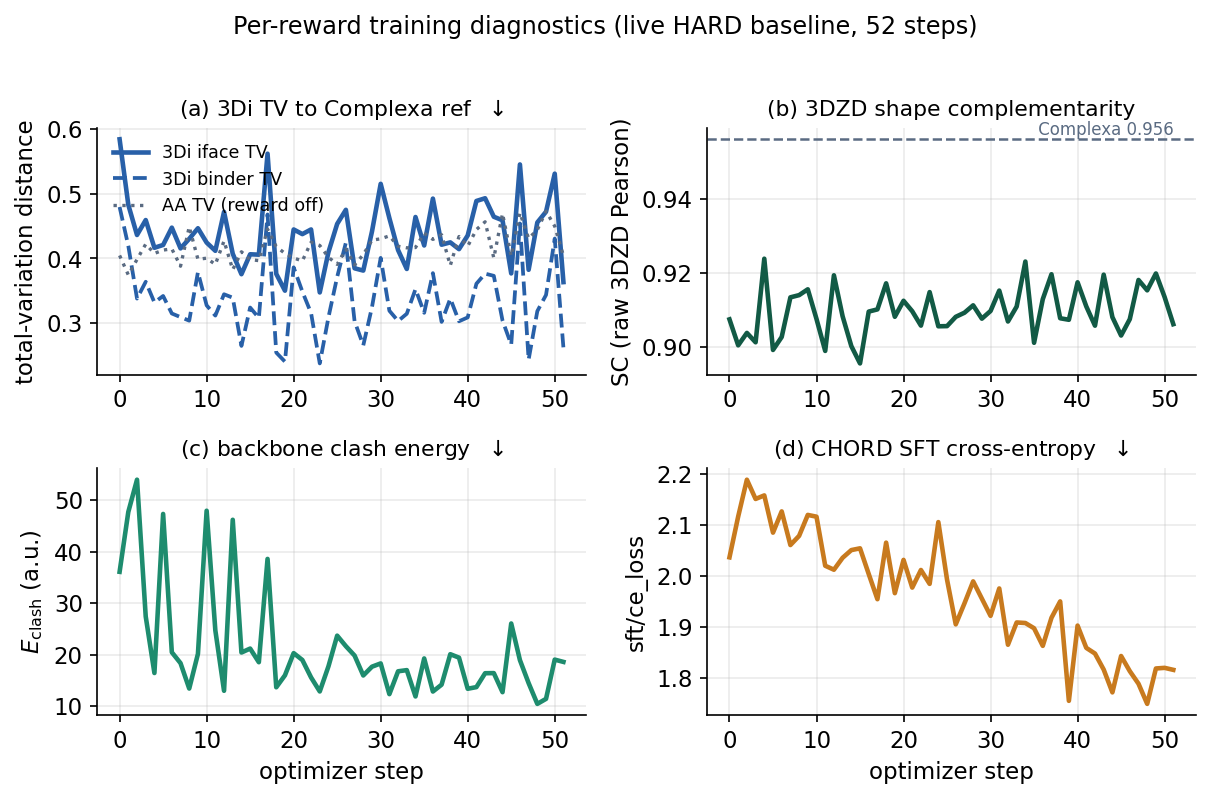
\includegraphics[width=0.98\linewidth]{figs/reward_diagnostics.png}
\caption{Per-reward training diagnostics (live HARD baseline, 52 optimizer steps).
\textbf{(a)} 3Di TV to the Complexa-38 reference falls for both interface and whole-binder
scopes, while AA TV (reward off) is flat --- the shift is specific to the optimized axis
(\S3.1). \textbf{(b)} 3DZD shape complementarity holds near the packed-backbone ceiling,
below the passing Complexa model (dashed, \S3.3). \textbf{(c)} backbone clash energy is driven
down (\S3.2). \textbf{(d)} CHORD SFT cross-entropy decreases as the sequence head distils the
LigandMPNN design (\S3.4).}
\label{fig:diag}
\end{figure}

\section{The second reward set: all-atom interface potentials}
\label{sec:potentials}
The active stack (\S3) scores the \emph{shape} of the packed interface ($\R_{\SC}$) but is blind to
its \emph{chemistry}: whether the packed side chains actually hydrogen-bond, salt-bridge, and pack
into a low-energy, well-buried interface. The second reward set closes this gap with classical
all-atom potentials evaluated on the \emph{same} LigandMPNN pack the shape reward already consumes
(\S2, pack branch) --- so it is Protenix-free and adds no train-time cost beyond a pack that is
already paid for. The terms are implemented self-contained in \ttk{scripts/\_packed\_potentials.py}
(NumPy $+$ biotite SASA; no PyRosetta/OpenMM dependency).

Three terms are proposed as rewards; write $\mathcal I$ for the set of heavy-atom pairs $(i,j)$ with
$i\in$ antigen, $j\in$ binder within the interface shell ($\le 5$\,\AA), and $r_{ij}=\lVert
x_i-x_j\rVert$.

\emph{Buried interface area.} $\R_{\Delta\mathrm{SASA}}=\mathrm{SASA}(\mathrm{ag})+
\mathrm{SASA}(\mathrm{bd})-\mathrm{SASA}(\mathrm{complex})$ (Shrake--Rupley), the total surface
area occluded on binding --- a monotone proxy for interface size and complementarity.

\emph{Interface hydrogen bonds.} A geometric count over donor/acceptor heavy-atom pairs, gated on
distance so it cannot be inflated by interpenetration:
\[
\R_{\mathrm{HB}}=\!\!\sum_{(d,a)\in\mathcal I}\!\!
   \mathbf 1\big[\,2.5\le r_{da}\le 3.5\,\text{\AA}\,\big],
\qquad
\R_{\mathrm{HB\text{-}sc}}\ \text{(side-chain donors/acceptors only).}
\]

\emph{Bounded packing energy.} A Rosetta-style Lennard--Jones split with a \emph{bounded} attractive
well and a capped repulsion, so an interpenetrated interface (small $r_{ij}$) cannot forge a large
favorable energy:
\[
\R_{\mathrm{LJ}}=-\!\!\sum_{(i,j)\in\mathcal I}\Big[\,
   \underbrace{\max\!\big(e_{ij},\,-\epsilon\big)}_{\text{atr, }\ge-\epsilon}
   +\underbrace{\min\!\big(e_{ij}+\epsilon,\,c_{\mathrm{rep}}\big)_{+}}_{\text{rep, capped}}\Big],
\qquad
e_{ij}=\epsilon\big[(r_0/r_{ij})^{12}-2(r_0/r_{ij})^{6}\big].
\]
Below the minimum ($r<r_0$) the attractive branch is clamped at $-\epsilon$ and the surplus is
routed into the capped repulsion term --- the fix that keeps a clash from reading as a $-10^{5}$
"favorable" contact. Each extensive term ships with a per-atom / per-residue density companion
(\ttk{hb\_density}, \ttk{e\_atr\_per\_atom}) so the reward cannot be won by simply enlarging the
interface.

\emph{Discriminator (offline).} We packed $3500$ Complexa-benchmark designs ($1008$ pass, $2492$
fail; $35$ targets) and scored every potential against the Protenix pass label. Table
\ref{tab:potentials} ranks them by AUROC. \textbf{Three all-atom potentials out-discriminate the
shipped $\R_{\SC}$ ($0.73$)}: total bounded LJ energy ($0.778$), buried $\Delta$SASA ($0.757$), and
interface H-bond count ($0.742$), each with a clean monotone quartile trend and a significant
logistic coefficient \emph{after} controlling for binder length and interface size --- so they are
not merely re-reading "how big is the interface." Two negative controls confirm the picture:
\ttk{n\_clash} is dead on packed complexes (AUROC $0.506$) because the packer has already resolved
steric clashes --- clash therefore belongs to a \emph{backbone} / per-token term (\S3.2, \S3.5),
never to the packed set --- and raw electrostatics ($0.549$) carries little signal once H-bonds and
packing are accounted for.

\begin{table}[htbp]
\centering
{\renewcommand{\arraystretch}{1.2}%
\begin{tabular}{@{}>{\raggedright\arraybackslash}p{5.9cm}
                    >{\centering\arraybackslash}p{1.4cm}
                    >{\centering\arraybackslash}p{1.2cm}
                    >{\centering\arraybackslash}p{2.0cm}
                    >{\centering\arraybackslash}p{3.0cm}@{}}
\toprule
\textbf{Potential (packed all-atom)} & \textbf{AUROC} & \textbf{dir} &
  \textbf{$\beta\,|\,$size} & \textbf{pass\% Q1$\rightarrow$Q4}\\
\midrule
\rowcolor{aTint}Bounded LJ energy $\R_{\mathrm{LJ}}$   & $0.778$ & $-$ & $-3.95$ & $60\!\rightarrow\!8$\\
\rowcolor{aTint}Buried $\Delta$SASA $\R_{\Delta\mathrm{SASA}}$ & $0.757$ & $+$ & $+2.72$ & $9\!\rightarrow\!61$\\
\quad LJ attractive only                              & $0.753$ & $-$ & $+0.38$ & $58\!\rightarrow\!9$\\
\rowcolor{aTint}Interface H-bonds $\R_{\mathrm{HB}}$   & $0.742$ & $+$ & $+0.36$ & $9\!\rightarrow\!56$\\
Side-chain H-bonds $\R_{\mathrm{HB\text{-}sc}}$        & $0.730$ & $+$ & $+0.60$ & $11\!\rightarrow\!50$\\
\midrule
3DZD shape complementarity $\R_{\SC}$ \emph{(shipped, \S3.3)} & $0.730$ & $+$ & --- & ---\\
\midrule
Salt bridges                                          & $0.674$ & $+$ & $+0.54$ & ---$\rightarrow\!42$\\
H-bond density                                        & $0.656$ & $+$ & $+0.32$ & $13\!\rightarrow\!44$\\
Packing (void proxy)                                  & $0.627$ & $+$ & $+0.05$ & $19\!\rightarrow\!41$\\
Buried unsat.\ polars                                 & $0.586$ & $+$ & $-0.43$ & $21\!\rightarrow\!36$\\
Electrostatics (Coulomb)                              & $0.549$ & $-$ & $-0.14$ & $34\!\rightarrow\!28$\\
Clash count \emph{(dead: packer resolves)}            & $0.506$ & $+$ & $-2.60$ & ---$\rightarrow\!34$\\
\bottomrule
\end{tabular}}
\caption{Offline predictiveness of the all-atom interface potentials on $3500$ LigandMPNN-packed
Complexa-benchmark designs ($1008$ pass / $2492$ fail, $35$ targets), scored against the Protenix
pass label. \textbf{AUROC} is direction-oriented (\textbf{dir} gives the favorable sign);
\textbf{$\beta\,|\,$size} is the standardized logistic coefficient after controlling for binder
length and interface-residue count; \textbf{pass\%} is the empirical pass rate in the bottom
vs.\ top score quartile. Highlighted rows (\textcolor{aTint}{\rule{1.6ex}{1.6ex}}) are the three
terms proposed as rewards --- each out-discriminates the shipped $\R_{\SC}$. As a yardstick, the
Protenix \ttk{iptm} scores AUROC $0.999$ (it partly defines the label). Computed by
\ttk{scripts/\_packed\_potentials\_analyze.py}.}
\label{tab:potentials}
\end{table}

\emph{Proposed integration.} Wire $\R_{\mathrm{LJ}}$ (bounded), $\R_{\Delta\mathrm{SASA}}$, and
$\R_{\mathrm{HB}}$ as the second reward set, each normalized by its per-atom density companion to
resist size-inflation, and keep salt bridges / packing / BUNS as tracked-but-ungraded diagnostics
(as \ttk{w\_sc\_clash} is today, \S3.3). The pack is amortized across the whole second set at no
marginal Protenix cost. Unlike $\R_{\SC}$ (a global descriptor correlation, no additive residue
split), these potentials admit an \emph{exact} per-token decomposition --- so they are delivered as
dense per-residue rewards, exactly like the per-token clash arm of \S3.5.

\subsection{Per-token form: dense all-atom interface credit}
\label{sec:pertoken-pot}
Each proposed potential is a sum over interface atom-pairs ($\R_{\mathrm{LJ}}$, $\R_{\mathrm{HB}}$)
or per-atom quantities ($\R_{\Delta\mathrm{SASA}}$), so --- exactly as the per-token clash arm of
\S3.5 splits the scalar clash energy per residue --- it decomposes onto the binder residue that owns
the binder-side atom. This turns each terminal scalar into a per-residue signal whose gradient lands
on the residues that actually make (or fail to make) the interface, rather than crediting every
structure token equally. The construction and the four-step GRPO plumbing are \emph{identical} to
\S3.5; only the per-residue score changes.

\textbf{1. Split each potential per residue (exact).} For potential $P\in\{\R_{\mathrm{LJ}},
\R_{\Delta\mathrm{SASA}},\R_{\mathrm{HB}}\}$ and design $i$, credit each interface pair/atom to its
binder residue $l$, giving $P^{(i,l)}$. For the pairwise terms this adds back exactly to the scalar,
$\sum_l P^{(i,l)}=P^{(i)}$; for $\R_{\Delta\mathrm{SASA}}$ the per-residue vector carries the
binder-side buried area (the antigen half is not creditable to a binder residue), which is precisely
the per-token binder reward wanted. Implemented in \ttk{scripts/\_packed\_potentials.py}
(\ttk{potentials\_per\_residue}); the exactness $\sum_l P^{(i,l)}=P^{(i)}$ is verified to machine
precision (max abs.\ error $\sim\!10^{-11}$; counts exact) over $800$ packed designs by
\ttk{scripts/\_packed\_potentials\_perres\_validate.py}.

\textbf{2--4. Per-residue advantage, design coupling, per-position surrogate.} Orient each potential
so higher $=$ better ($s_{i,l}=-\R_{\mathrm{LJ}}^{(i,l)}$ for energy; $s_{i,l}=+P^{(i,l)}$ for
$\R_{\Delta\mathrm{SASA}},\R_{\mathrm{HB}}$; multiple terms sum with weights $w_P$ into one
$s_{i,l}$), then apply the \emph{same} group-relative token-level normalization, design-advantage
coupling $A^{\text{struct}}_{i,l}=A_i+A^{\text{pot}}_{i,l}$, and per-position clipped structure
surrogate $\mathcal L^{\text{struct}}$ as \S3.5, Eqs.\ (per-token 2--4). The no-grad rollout
recompute gives $\ttk{ppo/struct\_ratio\_init}=1$ at the first inner iteration, the same correctness
guard.

\emph{Discriminator (offline).} The per-token signal survives the decomposition: aggregating each
per-residue vector by its mean over binder residues (the per-token-normalized quantity the dense
reward averages) and scoring against the Protenix pass label matches --- and for H-bonds exceeds ---
the extensive scalar (Table \ref{tab:pertokenpot}). This is the same offline gate that validated
$\R_{\SC}$ and the scalar potentials, now applied to the per-residue form.

\begin{table}[htbp]
\centering
{\renewcommand{\arraystretch}{1.2}%
\begin{tabular}{@{}>{\raggedright\arraybackslash}p{6.4cm}
                    >{\centering\arraybackslash}p{3.2cm}
                    >{\centering\arraybackslash}p{3.2cm}@{}}
\toprule
\textbf{Term (packed all-atom)} & \textbf{AUROC (per-token mean)} $\uparrow$ &
  \textbf{AUROC (scalar sum)}\\
\midrule
\rowcolor{aTint}Bounded LJ energy $\R_{\mathrm{LJ}}$       & $0.788$ & $0.785$\\
\rowcolor{aTint}Buried $\Delta$SASA $\R_{\Delta\mathrm{SASA}}$ & $0.758$ & $0.763$\\
\rowcolor{aTint}Interface H-bonds $\R_{\mathrm{HB}}$       & $0.751$ & $0.735$\\
Side-chain H-bonds $\R_{\mathrm{HB\text{-}sc}}$            & $0.744$ & $0.724$\\
Clash count \emph{(dead: packer resolves)}                & $0.529$ & $0.520$\\
\bottomrule
\end{tabular}}
\caption{Per-token decomposition retains offline predictiveness. On $800$ LigandMPNN-packed
Complexa-benchmark designs ($223$ pass / $577$ fail), \textbf{AUROC (per-token mean)} scores the
mean over binder residues of the per-residue vector; \textbf{AUROC (scalar sum)} scores its sum
(equal to the terminal scalar of Table \ref{tab:potentials}). The three graded terms
(\textcolor{aTint}{\rule{1.6ex}{1.6ex}}) hold their discrimination in per-residue form, and
per-residue normalization \emph{improves} the H-bond terms; \ttk{n\_clash} stays dead on packed
complexes --- confirming clash belongs to the backbone / per-token clash arm (\S3.5), not the packed
set. Computed by \ttk{scripts/\_packed\_potentials\_perres\_validate.py}.}
\label{tab:pertokenpot}
\end{table}

\subsection{Cross-arm interface energetics: where the current arms already sit}
\label{sec:crossarm-pot}
Table \ref{tab:potentials} asks whether a potential \emph{predicts} pass; Table
\ref{tab:crossarmpot} asks a different question --- \emph{where does each trained arm already sit} on
these same potentials, and how far is that from a real (native side-chain) interface. This is the
measurement that tells us which terms are safe to grade and which are reward-hackable. Every arm's
$\sim\!3800$ cold-offline A8 designs are re-packed with the \emph{same} LigandMPNN side-chain model
(uniform re-pack, \S2 pack branch) so the packer is not a confound across arms; the potentials are
then Table \ref{tab:potentials}'s exact terms.

\begin{table}[htbp]
\centering
\footnotesize
{\renewcommand{\arraystretch}{1.2}%
\setlength{\tabcolsep}{3.5pt}%
\begin{tabular}{@{}>{\raggedright\arraybackslash}p{2.55cm}
                    *{5}{>{\centering\arraybackslash}p{1.25cm}}
                    *{2}{>{\centering\arraybackslash}p{1.3cm}}@{}}
\toprule
 & \multicolumn{5}{c}{\textbf{GRPO arms (uniform LigandMPNN re-pack)}} &
   \multicolumn{2}{c}{\textbf{Complexa}}\\
\cmidrule(lr){2-6}\cmidrule(lr){7-8}
\textbf{Potential (dir)} & \textbf{Base} & \textbf{+AAR s75} & \textbf{exp-ctx s175} &
  \textbf{CHORD s100} & \textbf{CHORD s150} & \textbf{LMPNN} & \textbf{nat.\ SC}\\
\midrule
$\R_{\mathrm{LJ}}$ energy \ ($\downarrow$)   & $86.3$ & $26.4$ & $\mathbf{10.2}$ & $18.4$ & $15.6$ & $-27.8$ & $-34.6$\\
Electrostatics \ ($\downarrow$)              & $-7.8$ & $-9.6$ & $-9.6$ & $\mathbf{-14.3}$ & $-14.1$ & $-8.2$ & $-9.0$\\
Interface H-bonds \ ($\uparrow$)             & $\mathbf{16.5}$ & $10.7$ & $6.0$ & $9.2$ & $8.6$ & $6.6$ & $8.6$\\
Salt bridges \ ($\uparrow$)                  & $1.5$ & $1.5$ & $1.6$ & $\mathbf{2.3}$ & $2.2$ & $1.4$ & $1.7$\\
Buried $\Delta$SASA \ ($\uparrow$)           & $1994$ & $1881$ & $1397$ & $1934$ & $\mathbf{2051}$ & $1458$ & $1775$\\
Buried unsat.\ polars \ ($\downarrow$)       & $5.3$ & $5.1$ & $\mathbf{3.4}$ & $4.7$ & $4.9$ & $3.0$ & $3.7$\\
Clash count \ ($\downarrow$)                 & $74.0$ & $37.6$ & $\mathbf{20.6}$ & $31.9$ & $31.9$ & $2.6$ & $4.2$\\
Packing \ ($\uparrow$)                       & $\mathbf{9.3}$ & $8.0$ & $6.9$ & $7.2$ & $7.5$ & $6.4$ & $6.9$\\
\midrule
\emph{Iface residues (desc.)}                & $57.1$ & $51.3$ & $37.9$ & $52.1$ & $55.1$ & $38.1$ & $46.0$\\
\midrule
\multicolumn{8}{@{}l}{\emph{Backbone integrity (pre-pack; identical under either packing):}}\\
Chain-break \% \ ($\downarrow$)              & $28.1$ & $18.0$ & $18.8$ & $31.3$ & $30.2$ & \multicolumn{2}{c}{$0.5$}\\
\bottomrule
\end{tabular}}
\caption{\textbf{Cross-arm interface energetics.} Mean per-design potential for five Table-1 GRPO
arms ($n\!\approx\!3800$ designs each, cold A8 sampler) against the Complexa reference under
\emph{two} packings. All five GRPO arms and the \textbf{LMPNN} Complexa column ($n\!=\!3439$) are
re-packed with the \emph{same} LigandMPNN side-chain model, so the packer is not a confound; the
\textbf{nat.\ SC} column ($n\!=\!3500$) keeps Complexa's own generated side chains. \textbf{Bold}
marks the best value among the five GRPO arms in the favorable direction (dir). The bolding exposes
the reward-hack risk: \emph{Base}, the clashiest arm (clash $74$ vs Complexa $\sim\!3$,
$\R_{\mathrm{LJ}}\!=\!+86$), simultaneously \emph{maximizes} the extensive ``good'' terms --- H-bonds,
$\Delta$SASA, packing --- because it wins them by building the biggest, most interpenetrated
interface (iface residues $57$). \emph{expert-ctx s175} instead wins the clean terms
($\R_{\mathrm{LJ}}$, clash, BUNS) by \emph{shrinking} the interface (iface $38$, $\Delta$SASA
$1397$). \emph{CHORD s100/s150} are the best-balanced: a native-sized interface (iface $52$--$55$,
$\Delta$SASA $1934$--$2051$) with moderated clash and the best intensive chemistry (electrostatics
$-14.3$, salt bridges $2.3$); s100$\rightarrow$s150 grows the interface slightly and holds the
chemistry --- no energetic erosion. Every GRPO arm still carries $\sim\!5\text{--}28\times$ the
Complexa clash --- consistent with Table \ref{tab:potentials}: clash on the packed set is dead as a
reward and belongs to the backbone / per-token arm (\S3.2, \S3.5). \textbf{The two Complexa columns
answer the packer question:} re-packing Complexa's backbones with \emph{our} LigandMPNN model still
yields a strongly favorable $\R_{\mathrm{LJ}}=-27.8$ (vs native-SC $-34.6$) and near-zero clash
($2.6$ vs $4.2$) --- the same regime --- so the $\sim\!40$-unit LJ gap to our best arm is
\emph{intrinsic design headroom in the backbone}, not an artifact of Complexa keeping nicer native
side chains. The final row is a \emph{backbone} metric --- the fraction of designs with $\ge\!1$
broken C--N peptide bond (\ttk{chainbreak\_reward}, count gate) --- computed on the generated
backbone and hence pack-independent: Complexa is essentially break-free ($0.5\%$) while every GRPO
arm sits at $18\text{--}31\%$, and the dense CHORD seqtrack is the \emph{worst} ($31\%$, above base's
$28\%$), so no current reward controls it. This is the mirror of clash: clash is dead on the packed
set (Table \ref{tab:potentials}) but a broken backbone cannot be packed away, so chain-break is the
backbone-integrity term clash cannot be. Computed by \ttk{scripts/\_packed\_potentials\_compute.py}
$+$ \ttk{scripts/\_tab6\_energy\_separation.py} (potentials) and \ttk{scripts/\_tab6\_chainbreak.py}
(chain-break).}
\label{tab:crossarmpot}
\end{table}

\emph{Reward-design consequence.} Table \ref{tab:crossarmpot} sharpens the integration in
\S\ref{sec:pertoken-pot}. The two extensive ``area'' terms --- interface H-bonds and buried
$\Delta$SASA --- are \emph{maximized by the clashiest arm} (Base) and by the longest CHORD rollout
(s150), so grading their raw sums would reward interpenetration and interface bloat, the exact
failure the bounded $\R_{\mathrm{LJ}}$ was built to resist. They are therefore graded only through
their per-atom \emph{density} companions (\S\ref{sec:pertoken-pot}), or demoted to tracked
diagnostics. The bounded $\R_{\mathrm{LJ}}$ is the primary graded term: its sign is unambiguous
(both Complexa packings $\approx\!-30$ vs all five arms positive), it cannot be won by
interpenetration, and no arm has reached a favorable value --- the uniform-repack column proves the
$\sim\!40$-unit gap is real backbone headroom, not packing, so the reward carries genuine,
non-saturated gradient. The intensive chemistry terms (electrostatics, salt bridges), where CHORD
already edges past both Complexa packings, are the low-risk secondary rewards. This is the direct
evidence for grading $\R_{\mathrm{LJ}}$ (density-normalized) as the primary second-set reward with
$\R_{\Delta\mathrm{SASA}}$/$\R_{\mathrm{HB}}$ entering only in density form. Finally, the chain-break
row identifies a \emph{backbone} bucket the interface potentials cannot cover: no arm controls
peptide-bond integrity (CHORD is worst at $31\%$ vs Complexa's $0.5\%$), so the next run pairs the
packed interface-energy set with a backbone / per-token structure set --- per-token clash \emph{and}
a graded chain-break term (\ttk{chainbreak\_reward}, \S3.2/\S3.5) --- since chain-break survives the
pack exactly where clash does not.

\section{The third reward set: Protenix fold-consistency distillation}
\label{sec:protenix-sft}
Every reward so far is computed on structure the policy \emph{itself} emitted --- the generated
backbone (\S3.2, \S3.5), its LigandMPNN pack (\S3.3, \S4), or its 3Di tokens (\S3.1). None of them
can tell the policy that the structure it drew is not the structure its own sequence \emph{folds
into}. The diagnostic that exposes this is the fold/dock split of \S3.4: refolding the step-50 arm
with Protenix reproduces the binder \emph{monomer} fold (binder-only C$\alpha$-RMSD median
$2.4$\,\AA) but disagrees on the \emph{docking pose} (antigen-aligned binder L-RMSD median
$29.5$\,\AA). The high ipTM is Protenix's confidence in \emph{an} interface, not the generated one.
No backbone-, pack-, or 3Di-histogram reward can move this, because none of them sees where the
sequence \emph{wants} to dock --- \textbf{docking-pose fidelity is the clearest open lever, and it is
a property of the sequence$\to$structure map, not of any quantity read off the generated pose.}

\textbf{The idea: the exact structural dual of CHORD (\S3.4).} CHORD distils the LigandMPNN
\emph{design} branch --- the sequence-given-structure conditional $q(a^{\ast}\!\mid\!X,T)$ --- into
the \ttk{sequence} track. Its mirror image is a \emph{fold} branch: run the policy's own output
sequence through Protenix (the same oracle that scores the benchmark) to predict the complex
structure $X^{\ast}\!\sim\!\mathcal P(a,T,E)$, then distil that structure into the two structural
tracks the policy denoises. This is the missing second arrow of the round-trip: \S2 added the
\emph{design} branch $\mathrm{MPNN}(X)\!\to\!a^{\ast}$ (sequence expert); we now add the \emph{fold}
branch $\mathrm{Protenix}(a)\!\to\!X^{\ast}$ (structure expert), whose fixed point is a policy whose
generated structure \emph{is} what its sequence folds and docks to.

\begin{center}
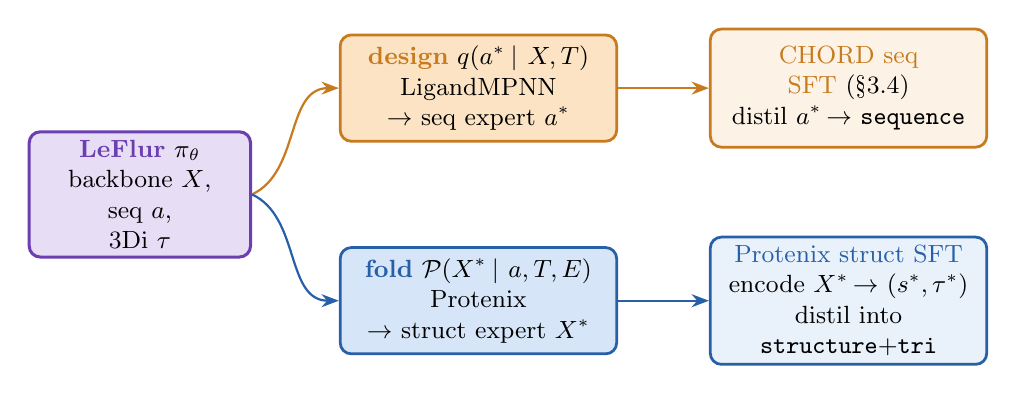
\begin{tikzpicture}[x=1cm,y=1cm,font=\small,>={Stealth[length=2.2mm]},
  core/.style={draw=lfLine,line width=1.1pt,rounded corners,align=center,text width=2.6cm,minimum height=1.25cm,inner sep=3pt,fill=lfFill},
  mp/.style  ={draw=ioLine,line width=1.0pt,rounded corners,align=center,text width=2.9cm,minimum height=1.3cm,inner sep=3pt,fill=ioFill},
  ds/.style  ={draw=bLine,line width=1.0pt,rounded corners,align=center,text width=3.3cm,minimum height=1.35cm,inner sep=3pt,fill=bFill},
  fd/.style  ={draw=dLine,line width=1.0pt,rounded corners,align=center,text width=3.3cm,minimum height=1.35cm,inner sep=3pt,fill=dFill},
  rwB/.style ={draw=bLine,line width=1.0pt,rounded corners,align=center,text width=3.3cm,minimum height=1.5cm,inner sep=3pt,fill=bTint},
  rwD/.style ={draw=dLine,line width=1.0pt,rounded corners,align=center,text width=3.3cm,minimum height=1.5cm,inner sep=3pt,fill=dTint},
  flow/.style={->,thick}]
\node[core] (lf)  at (0.0, 0.0) {\textbf{\textcolor{lfLine}{LeFlur} $\pi_\theta$}\\ backbone $X$,\\ seq $a$,\\ 3Di $\tau$};
\node[ds]   (ds)  at (4.3, 1.35){\textbf{\textcolor{bLine}{design}} $q(a^{\ast}\!\mid X,T)$\\ LigandMPNN\\ $\to$ seq expert $a^{\ast}$};
\node[fd]   (fd)  at (4.3,-1.35){\textbf{\textcolor{dLine}{fold}} $\mathcal P(X^{\ast}\!\mid a,T,E)$\\ Protenix\\ $\to$ struct expert $X^{\ast}$};
\node[rwB]  (rB)  at (9.0, 1.35){\textcolor{bLine}{CHORD seq SFT}\ (\S3.4)\\ distil $a^{\ast}\!\to$ \ttk{sequence}};
\node[rwD]  (rD)  at (9.0,-1.35){\textcolor{dLine}{Protenix struct SFT}\\ encode $X^{\ast}\!\to(s^{\ast},\tau^{\ast})$\\ distil into \ttk{structure}$+$\ttk{tri}};
\draw[flow,bLine] (lf.east) to[out=25,in=180]  (ds.west);
\draw[flow,dLine] (lf.east) to[out=-25,in=180] (fd.west);
\draw[flow,bLine] (ds) -- (rB);
\draw[flow,dLine] (fd) -- (rD);
\end{tikzpicture}
\end{center}

\textbf{Encoding the oracle structure into both structural tracks.} Protenix returns an all-atom
complex; we parse its binder chain to an atom14 backbone and run the \emph{same} encoders the policy
was trained against, so the expert targets live in exactly the policy's own vocabularies:
\begin{itemize}
\item \textbf{LG / \ttk{structure\_tokens}} --- the backbone-geometry codec tokens $s^{\ast}$ (the
  fold), from the discrete local-geometry encoder;
\item \textbf{3Di / \ttk{tri\_tokens}} --- the 3Di structural-alphabet tokens $\tau^{\ast}$, from the
  3Di encoder (the \ttk{encode}-path tokenizer),
\end{itemize}
both defined per binder residue and aligned $1{:}1$ with the policy's generated positions. Deriving
\emph{both} tracks from the one Protenix structure (rather than only the fold, or only 3Di) is what
makes the target a self-consistent structure the policy can actually reach on both of its structural
heads.

\textbf{The distillation term (identical machinery to \S3.4).} Let $p^{s}_{s,l}=\pi_\theta(s^{\ast}_l
\!\mid\!x_{t_s})$ and $p^{\tau}_{s,l}=\pi_\theta(\tau^{\ast}_l\!\mid\!x_{t_s})$ be the policy's
structure- and tri-endpoint probabilities of the Protenix-derived expert token at supervised step
$s$, position $l$, evaluated --- as in CHORD --- on the policy's \emph{own} noised trajectory states
(DAgger: the fold oracle is queried on the learner's sequence). With the same $\phi$-weighting
$\phi=p(1-p)$ (detached) that zeroes consensus and rejected tokens, and the same masked-only,
whole-binder scope, the structure SFT loss is the token-CE toward the oracle tokens, summed over the
two structural tracks:
\[
\mathcal L_{\text{SFT-}\phi}^{\text{struct}}
   =\frac1{|S|}\sum_{s\in S}
     \Big[\,w_s\,\ell^{\,s}_s(s^{\ast})\;+\;w_\tau\,\ell^{\,\tau}_s(\tau^{\ast})\,\Big],
\qquad
\mathcal L=(1-\mu)\mathcal L_{\mathrm{GRPO}}+\mu_{\text{seq}}\mathcal L_{\text{SFT}}^{\text{seq}}
   +\mu_{\text{str}}\mathcal L_{\text{SFT-}\phi}^{\text{struct}},
\]
each $\ell_s$ the $\phi$-weighted CE of Eq.\ (\S3.4). Because the target is the expert
\emph{structure}, the natural context for the endpoint forward is the expert's own structural tokens
(the $s^{\ast},\tau^{\ast}$ of $X^{\ast}$) at revealed positions --- exactly the expert-context fix
that \S3.4 applies on the sequence side (\ttk{\_expert\_context\_seq}), here on the structure/tri
tracks --- so the distilled conditional is $p_\theta(X^{\ast}\!\mid\!X^{\ast}\text{-context},a,T)$,
whose fixed point is the Protenix fold-and-dock, not a policy/oracle chimera.

\textbf{Why not just the terminal scalar.} A scalar consistency reward (generated-vs-Protenix
complex RMSD, or a TM/lDDT agreement) is available and will be tracked, but --- as for AAR vs.\ CHORD
(\S3.4) --- a single number is a weak signal for a per-residue structure-prediction target and
credits every structure token equally. The dense form lands the gradient on the residues whose
generated geometry disagrees with the fold, which is where the docking-pose error concentrates.

\emph{Protenix is used here as a structure oracle, not a confidence reward.} Consistent with the
rest of the stack (all \ttk{iptm}/\ttk{ptm}/\ttk{plddt} terms are ungraded offline labels), we
distil Protenix's predicted \emph{coordinates} --- never its scalar confidence --- into the policy.

\subsection{Docking correctness: relabeled conditioning $+$ a dock reward}
\label{sec:dock}
The fold/dock split has a second consequence for the SFT above. Generation conditions on a specified
epitope $E$ (bidirectional hotspot conditioning $+$ epitope CFG, \S1), but Protenix routinely docks
the policy sequence at a \emph{different} site $E'\!\neq\!E$ (the $29.5$\,\AA\ antigen-aligned
L-RMSD; the high ipTM is confidence in \emph{an} interface, not the requested one). The structure SFT
as described conditions its endpoint forward on the originally-specified $E$ while the target
$X^{\ast}$ realizes $E'$ --- distilling the inconsistent conditional $p(\text{structure}@E'\mid
\text{cond}{=}E)$, the exact conditioning-side analogue of the sequence-context chimera fixed in
\S3.4. We fix it the same way, and add the missing on-target pressure as a separate scalar, both off
\emph{one} shared primitive so no extra fold is spent.

\textbf{Shared primitive: the achieved interface from $X^{\ast}$.} From the Protenix complex derive
the interface the sequence actually made, by heavy-atom contact (cutoff $\approx\!5$\,\AA):
$E'$ $=$ antigen residues contacting the binder, $P'$ $=$ its binder-side dual
(\ttk{derive\_interface\_from\_structure}, placed beside the $s^{\ast}/\tau^{\ast}$ encoders). Both
changes below read this one contact set.

\textbf{Relabel the SFT conditioning ($E\!\to\!E'$).} Rebuild the conditioning tensor from
$(E',P')$ --- the identical construction to the generation path --- and condition the structure-SFT
endpoint forward on it (a \ttk{conditioning\_override} on the endpoint call; the single edit point
that today reads \ttk{static["conditioning\_tensor"]} unchanged). The SFT then trains
$p_\theta(\text{structure}@E'\mid\text{cond}{=}E')$ --- a proper function of the conditioning that
generalizes back to the requested epitope at inference ($\text{cond}{=}E\!\to\!\text{structure}@E$).
Every design is kept (no dock-gate, no discarded data) and the target is always self-consistent. This
is \emph{coherence} supervision; it does not by itself make the policy dock where we asked.

\textbf{The dock reward $\R_{\mathrm{dock}}$ (scalar).} On-target docking is the orthogonal signal,
supplied by a scalar term on the same fold. For the specified epitope $E$, the $X^{\ast}$
contacted-antigen set $\mathcal C$, and $d_e$ the minimum distance from antigen residue $e$ to any
binder heavy atom,
\[
r_{\mathrm{rec}}=\frac1{|E|}\sum_{e\in E}\sigma\!\Big(\tfrac{d_0-d_e}{w}\Big),
\qquad
r_{\mathrm{prec}}=\frac{|\,\mathcal C\cap E\,|}{|\mathcal C|},
\qquad
\R_{\mathrm{dock}}=\frac{2\,r_{\mathrm{rec}}\,r_{\mathrm{prec}}}{r_{\mathrm{rec}}+r_{\mathrm{prec}}}
\in[0,1],
\]
with $d_0\!\approx\!5\text{--}8$\,\AA\ and $w\!\approx\!1\text{--}2$\,\AA. Soft recall rewards
\emph{actually touching} the requested residues (a dense gradient, not a $0/1$ indicator); soft
precision is the anti-smear guard --- it stops the policy from wrapping the whole antigen to trivially
cover $E$; their harmonic mean penalizes both misses and smearing. $\R_{\mathrm{dock}}$ enters the
GRPO objective as a standard group-relative (Dr.GRPO) scalar at weight $w_{\mathrm{dock}}$, alongside
clash/shape/3Di-TV. It is the on-target counterpart to ipTM: ipTM says ``there is a confident
interface,'' $\R_{\mathrm{dock}}$ says ``it is the one we asked for'' --- putting the epitope
objective in the \emph{gradient} rather than leaning on inference-time CFG. Pass
($\text{pTM}\!>\!0.8\wedge\text{ipTM}\!>\!0.7$) stays an offline label.

\textbf{Division of labor and guards.} The two signals are orthogonal: a coherent-but-off-target
design keeps full (relabeled) SFT credit yet earns low $\R_{\mathrm{dock}}$; an
on-target-but-incoherent design earns high $\R_{\mathrm{dock}}$ yet low SFT --- together they pull
toward coherent \emph{and} on-target. Because the relabel lets the SFT happily teach coherent
\emph{off}-target folds, $w_{\mathrm{dock}}$ must be strong enough to counter it (too weak and the
policy drifts off-epitope). The precision term and the co-active clash/shape rewards guard the
interpenetration/smear failure mode of \S3.2; $\R_{\mathrm{dock}}$ may optionally be gated by a
minimum pTM so it never credits a garbage fold that happens to touch $E$. \emph{Caveat:} it trusts
Protenix's docked pose and inherits its pose noise, mitigated by multi-seed averaging. As with every
reward before it enters the gradient, $\R_{\mathrm{dock}}$ is first validated offline --- it must
separate passing-Complexa complexes from off-epitope generations.

\textbf{Cost and integration.} Unlike the first two reward sets, this one is \emph{not} amortized on
the free pack: it spends one Protenix fold per supervised design --- and the relabel and
$\R_{\mathrm{dock}}$ both reuse \emph{that same} fold, at zero extra fold cost. The worker-pool $+$
client that already serve the offline label (\ttk{scripts/protenix\_reward\_server.py}) are reused;
the term is gated behind its own \ttk{N\_WORKERS}$>0$ and a subsample fraction (fold a fraction of the
group, cache by sequence) so the fold budget is a tunable knob rather than a per-rollout tax. It is
proposed as the third set precisely because it buys the one axis the Protenix-free sets cannot --- the
dock --- at a Protenix-in-the-loop price.

\emph{Implementation status.} The structure-SFT distillation term
($\mu_{\text{str}},w_s,w_\tau,\phi$, expert-context, masked-only) is code-complete and wired live in
the trainer, config-reachable, and covered by unit tests; the first fresh-\ttk{OUTBASE} run with
$\mu_{\text{str}}{>}0$ is being launched. The docking additions of this subsection --- the shared
$X^{\ast}$-interface primitive, the conditioning relabel, and $\R_{\mathrm{dock}}$ --- are fully
specified (\ttk{docs/leflur/grpo\_dock\_correctness\_reward\_plan.md}) and are the next increment,
not yet wired.

\section{From reward to gradient}
All rewards act through GRPO on the \emph{same} stored rollout trajectory. Each inner PPO
iteration draws one step subset $S=\{s_1,\dots,s_k\}$, $k=\ttk{steps\_per\_update}=3$, uniformly
from the $40$ steps (\ttk{\_sample\_step\_subset}); both the policy log-prob and the CHORD CE are
evaluated on this \emph{same} $S$.

\textbf{Differentiable transition log-prob.} Every reward gradient flows through the probability the
policy assigned to the moves it actually sampled. We rebuild that probability from the stored head
logits differentiably (\ttk{dfm\_step\_logprob}), reproducing the absorbing-state discrete
flow-matching (DFM) sampler out-of-place so gradients reach the logits.

Fix one track and one denoising step, from time $t\in[0,1)$ to $t+\mathrm dt$ ($\mathrm dt$ the step
size). For position $l$ let $z_l$ be the model's logits over the vocabulary (predicting the
\emph{clean} token, mask column set to $-\infty$); $T$ the sampling temperature; $\eta$ the
stochasticity; $\mathbb 1^{\mathrm{msk}}_l=[x_{t,l}{=}\text{mask}]$ the indicator that $l$ is
currently masked; and $p^{(1)}_l=\mathrm{softmax}(z_l/T)$ the predicted clean-token distribution.
The unnormalized transition weights $\tilde q_l$ over the vocabulary have two parts --- \emph{unmask}
a masked position toward a clean token, or (before the final step) \emph{remask} an unmasked one:
\[
\tilde q_l \;=\;
\underbrace{\mathrm dt\,\frac{1+\eta t}{1-t}\,p^{(1)}_l\;\mathbb 1^{\mathrm{msk}}_l}_{\text{unmask}}
\;+\;
\underbrace{\mathrm dt\,\eta\,e_{\text{mask}}\,\big(1-\mathbb 1^{\mathrm{msk}}_l\big)\,\mathbb 1[t{+}\mathrm dt<1]}_{\text{remask}},
\]
where $e_{\text{mask}}$ is the one-hot vector on the mask token. Regularizing
($q_l=\mathrm{reg}(\tilde q_l)$: clamp to $[0,1]$, then place the leftover mass on the ``stay-put''
self-transition at $x_{t,l}$) makes each $q_l$ a proper transition distribution. The sampler draws
from the row-normalized $q_l$, so the log-probability of the sampled trajectory --- summed over the
step subset $S$, its tracks $\tau$, and the generated positions $\mathrm{gen}^\tau$ of each track
(fixed/inpainted positions excluded) --- is
\[
\log\pi_\theta(S)=\sum_{s\in S}\ \sum_{\tau}\ \sum_{l\in\mathrm{gen}^\tau}
   \log\frac{q_l\!\big(x_{t+\mathrm dt,\,l}\big)}{\sum_{v} q_l(v)} ,
\]
with $x_{t+\mathrm dt,l}$ the token actually sampled at that position and $v$ ranging over the
vocabulary. \emph{Two callers, one kernel:} GRPO evaluates it on the \emph{biased} logits the sampler
actually drew from (classifier-free guidance $+$ inference bias, via
\ttk{\_recompute\_biased\_step\_logits}); CHORD's SFT term uses the \emph{raw conditional}
sequence-endpoint logits (no CFG/bias, via \ttk{\_sft\_seq\_endpoint\_logits}).

\textbf{Scalar advantage and clipped surrogate.} A design's scalar reward $r_i$ (the weighted sum
of the three scalar terms above) becomes a group-relative advantage, and that one number
multiplies the design's entire summed log-prob:
\[
A_i=\frac{r_i-\bar r}{\sigma_r+\epsilon}\ \ (\ttk{normalize\_advantage}),
\qquad
\rho_i=\exp\!\big(\log\pi_\theta^{(i)}(S)-\log\pi_{\theta_{\mathrm{old}}}^{(i)}(S)\big),
\]
\[
\mathcal L_{\mathrm{GRPO}}=-\frac1G\sum_i\min\!\big(\rho_i A_i,\ \mathrm{clip}(\rho_i,1{\pm}\varepsilon)\,A_i\big),
\qquad G=\ttk{group\_size}=64 .
\]
The no-grad snapshot $\log\pi_{\theta_{\mathrm{old}}}$ gives $\rho_i\!\approx\!1$ at the first
inner iteration (\ttk{ppo/ratio\_init}). The two dense terms add to this: CHORD via the
$\mu$-blend, per-token clash via the added per-position surrogate.

\subsection{Update schematic}
The GRPO log-prob path (teal) and the CHORD SFT path (amber) fork off the \emph{same} shared step
subset $S$ and rejoin in the convex-blend loss. (Shown as two branches for clarity; the fast path
fuses them into one forward.)

\begin{center}
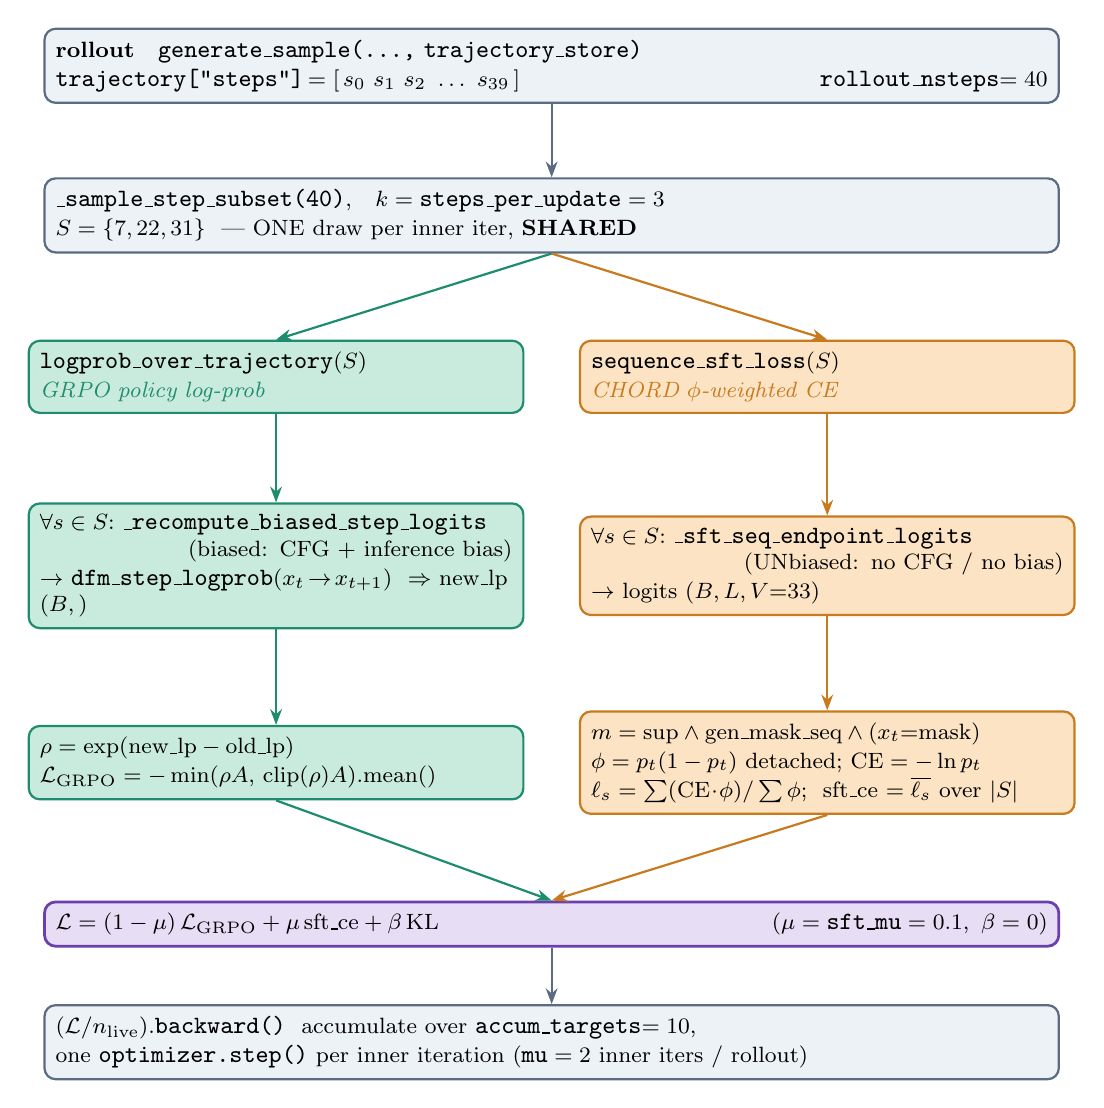
\begin{tikzpicture}[font=\footnotesize,>={Stealth[length=2mm]},
  data/.style={draw=ioLine,fill=ioFill,line width=0.8pt,rounded corners,align=left,inner sep=4pt,text width=12.6cm},
  grpo/.style={draw=aLine,fill=aFill,line width=0.8pt,rounded corners,align=left,inner sep=4pt,text width=6.0cm},
  sft/.style ={draw=bLine,fill=bFill,line width=0.8pt,rounded corners,align=left,inner sep=4pt,text width=6.0cm},
  comb/.style={draw=lfLine,fill=lfFill,line width=1.0pt,rounded corners,align=left,inner sep=4pt,text width=12.6cm},
  fl/.style={->,thick,ioLine},flA/.style={->,thick,aLine},flB/.style={->,thick,bLine}]

\node[data] (roll) at (3.5, 0)
  {\textbf{rollout}\quad\ttk{generate\_sample(..., trajectory\_store)}\\[1pt]
   \ttk{trajectory["steps"]}\,$=[\,s_0\ s_1\ s_2\ \dots\ s_{39}\,]$\hfill\ttk{rollout\_nsteps}$=40$};
\node[data] (sub) at (3.5,-1.9)
  {\ttk{\_sample\_step\_subset(40)},\quad$k=\ttk{steps\_per\_update}=3$\\[1pt]
   $S=\{7,22,31\}$\ \ \textemdash\ ONE draw per inner iter, \textbf{SHARED}};

\node[grpo] (lp) at (0,-3.95)
  {\ttk{logprob\_over\_trajectory}$(S)$\\[1pt]\textcolor{aLine}{\itshape GRPO policy log-prob}};
\node[sft]  (sf) at (7,-3.95)
  {\ttk{sequence\_sft\_loss}$(S)$\\[1pt]\textcolor{bLine}{\itshape CHORD $\phi$-weighted CE}};

\node[grpo] (lpc) at (0,-6.35)
  {$\forall s\in S$:\ \ttk{\_recompute\_biased\_step\_logits}\\ \hfill(biased: CFG $+$ inference bias)\\[1pt]
   $\to$ \ttk{dfm\_step\_logprob}$(x_t\!\to\!x_{t+1})$\ \ $\Rightarrow$\ new\_lp $(B,)$};
\node[sft]  (sfc) at (7,-6.35)
  {$\forall s\in S$:\ \ttk{\_sft\_seq\_endpoint\_logits}\\ \hfill(UNbiased: no CFG / no bias)\\[1pt]
   $\to$ logits $(B,L,V{=}33)$};

\node[grpo] (lpr) at (0,-8.85)
  {$\rho=\exp(\text{new\_lp}-\text{old\_lp})$\\[1pt]
   $\mathcal L_{\mathrm{GRPO}}=-\min(\rho A,\,\mathrm{clip}(\rho)A).\mathrm{mean}()$};
\node[sft]  (sfr) at (7,-8.85)
  {$m=\mathrm{sup}\wedge\mathrm{gen\_mask\_seq}\wedge(x_t{=}\text{mask})$\\[1pt]
   $\phi=p_t(1-p_t)$ detached;\ $\mathrm{CE}=-\ln p_t$\\[1pt]
   $\ell_s=\sum(\mathrm{CE}\!\cdot\!\phi)/\sum\phi$;\ \ sft\_ce $=\overline{\ell_s}$ over $|S|$};

\node[comb] (loss) at (3.5,-10.9)
  {$\mathcal L=(1-\mu)\,\mathcal L_{\mathrm{GRPO}}+\mu\,\text{sft\_ce}+\beta\,\mathrm{KL}$
   \hfill$(\mu=\ttk{sft\_mu}=0.1,\ \beta=0)$};
\node[data] (bwd) at (3.5,-12.4)
  {$(\mathcal L/n_{\mathrm{live}}).\ttk{backward()}$\ \ accumulate over \ttk{accum\_targets}$=10$,\\[1pt]
   one \ttk{optimizer.step()} per inner iteration\ ($\ttk{mu}=2$ inner iters / rollout)};

\draw[fl] (roll) -- (sub);
\draw[flA] (sub.south) -- (lp.north);
\draw[flB] (sub.south) -- (sf.north);
\draw[flA] (lp) -- (lpc);  \draw[flB] (sf) -- (sfc);
\draw[flA] (lpc) -- (lpr); \draw[flB] (sfc) -- (sfr);
\draw[flA] (lpr.south) -- (loss.north);
\draw[flB] (sfr.south) -- (loss.north);
\draw[fl] (loss) -- (bwd);
\end{tikzpicture}
\end{center}

When \ttk{per\_token\_clash} is on, the \ttk{struct} track is removed from the left (GRPO) box and
gets its own per-position surrogate $\mathcal L^{\text{struct}}$ (\S3.5), added into
$\mathcal L_{\mathrm{GRPO}}$ before the blend; \ttk{seq}$+$\ttk{tri} keep the scalar-advantage
path shown.

\section{Live training configuration}
Both live arms share: Dr.GRPO-style update, warm-start \ttk{leflur-binder-3di}, $G{=}64$,
\ttk{rollout\_nsteps}$=40$, \ttk{steps\_per\_update}$=3$, \ttk{mu}$=2$ inner iters,
\ttk{accum\_targets}$=10$ (gradient averaged over 10 targets/step), lr $10^{-5}$,
$\beta{=}0$ (KL off), \ttk{eps\_clip}$=0.2$, gradient checkpointing on, epitope conditioning on,
\ttk{sequence\_diversity\_penalty}$=2$, \ttk{tri\_diversity\_penalty}$=8$. \emph{These last two are
\textbf{sampler}-side per-design frequency penalties applied during rollout generation, not reward
terms}; the reward-side diversity weights (\ttk{w\_seq\_diversity}, \ttk{w\_struct\_diversity}) and the
proposed \ttk{w\_seq\_hamming} were all $0$, so between-design diversity was \emph{logged but never
graded} in the runs to date --- the collapse of \S\ref{sec:seqcomplex} is what a nonzero reward-side
term is meant to address. Protenix is off
(\ttk{N\_WORKERS}$=0$); a separate A10G repack array serves the pack/design pool. Active reward
weights: \ttk{w\_3di\_dist}$=1$, \ttk{w\_clash\_contact}$=1$, \ttk{w\_shape}$=1$,
\ttk{sft\_mu}$=0.1$; the per-token fork adds \ttk{per\_token\_clash}$=$true,
\ttk{w\_pt\_clash}$=1$, \ttk{pt\_clash\_tracks}$=$\ttk{[structure\_tokens]}.

\textbf{Degeneracy watch.} A rising interface AAR together with an AA distribution racing away from the
Complexa reference (\ttk{dist/tv\_aa}, observed to climb $0.42\!\to\!0.59$ over the CHORD run) and a
falling per-design complexity ($\overline{\mathrm{LC}}$, \S\ref{sec:seqcomplex}) is the degenerate
outcome and kills an arm. \emph{Between-design novelty is not a reliable watch}:
\ttk{diversity/seq\_novelty\_mean} held $\approx\!0.91$ throughout the same run --- it is blind to
per-design collapse (\S\ref{sec:seqcomplex}). Health keys: \ttk{sft/ce\_loss} (should fall),
\ttk{dist/tv\_aa} (should not race away), $\overline{\mathrm{LC}}$/$\bar h$ (should not fall),
\ttk{ppo/grad\_norm} (SFT must not swamp the policy gradient), and for the per-token arm
\ttk{ppo/struct\_ratio\_init}$\approx1$, \ttk{ptclash/adv\_abs\_mean}.

\section{Deliverable: a self-contained protein-RL post-training package}
\label{sec:package}
Everything above is \emph{one} instantiation --- a LeFlur binder policy against a specific reward
stack --- of a general capability: \textbf{post-training a token-based protein design model with GRPO
against composable, physically-grounded rewards, using differentiable trajectory log-probs and
out-of-process reward oracles}. Packaging that capability so a practitioner can \ttk{pip install} it
and post-train \emph{their own} protein language model or latent-structure-token model --- without
importing LeFlur, LBSTER, or our SLURM harness --- is a first-class deliverable. This section maps
what is already reusable, the couplings that must be cut, and the small set of interfaces that turn
the current code into an importable framework (working name \ttk{plm-design-rl}).

\subsection{What is already reusable}
The machinery is already largely factored into pure, dependency-light layers; the packaging work is
mostly \emph{declaring interfaces around them}, not rewriting them.
\begin{itemize}
\item \textbf{Reward terms} --- \ttk{lobster.rl\_training.rewards}. Every term (clash, chain-break,
  interface-distribution, diversity/linguistic-complexity, 3DZD shape complementarity, AAR, all-atom
  potentials, self-consistency TM, Protenix client) is a \emph{pure} numpy/torch module with no
  \ttk{trl} import and no dependency on the trainer loop --- the subpackage docstring already
  enforces this discipline (``\emph{Each module is pure \dots\ so the policy side can import the
  reward terms without pulling in the reward oracle's heavy deps}''). They are plain functions
  (\ttk{chainbreak\_reward}, \ttk{distribution\_terms}, \ttk{shape\_complementarity\_reward\_atoms},
  \ttk{lc\_saturating\_reward}), so the reward layer is \emph{already} a library.
\item \textbf{The differentiable log-prob kernel} --- \ttk{lobster.rl\_training.\_dfm\_logprob}
  (\ttk{dfm\_step\_prob} / \ttk{dfm\_step\_logprob} / \ttk{dfm\_step\_kl}). This rebuilds the
  absorbing-state discrete-flow-matching transition distribution out-of-place so gradients reach the
  head logits (``From reward to gradient'', \S\ref{sec:package} above). It is pure
  torch\,$+$\,bionemo --- the reusable ``differentiate the log-prob of a sampled generation'' engine.
\item \textbf{The trainer as configuration} --- \ttk{GRPOTrainerConfig} is already a declarative
  surface (per-term weights, per-metric clips, the CHORD $\mu$-blend, the per-token toggles, and the
  optimization knobs $G$/\ttk{rollout\_nsteps}/\ttk{mu}/\ttk{lr}/\ttk{eps\_clip}/\ttk{accum\_targets});
  \ttk{LeFlurGRPOTrainer} composes the reward client, the diversity terms, and the log-prob/KL
  kernels; \ttk{TargetSpec} declares one design target.
\item \textbf{The oracle transport} --- \ttk{ShapeRewardClient} (\ttk{submit\_group} /
  \ttk{collect\_group} / \ttk{rewards\_for\_group}) $+$ \ttk{scripts/ligandmpnn\_repack\_server.py}
  is a working async submit/block queue over a shared filesystem, with atomic-rename claiming so a
  worker pool of any size cooperates without coordination. This is the reusable pattern for running
  a heavy scorer (LigandMPNN, Protenix, ProteinMPNN) on its own accelerators off the policy's GPU.
\end{itemize}

\subsection{The couplings to cut}
Four things currently prevent ``import and post-train my model'':
\begin{itemize}
\item \textbf{The policy contract is implicit.} The trainer calls LeFlur methods \emph{by name}
  (\ttk{rollout\_with\_logprobs}, \ttk{\_recompute\_biased\_step\_logits},
  \ttk{logprob\_over\_trajectory}, \ttk{sequence\_sft\_loss},
  \ttk{logprob\_and\_sft\_over\_trajectory}) and hard-codes LeFlur's three tracks and their
  per-track vocab / mask-index conventions. No other model can be dropped in because there is no
  declared interface to implement.
\item \textbf{The log-prob is sampler-specific.} \ttk{\_dfm\_logprob} is correct for
  absorbing-state masked diffusion but not for autoregressive decoders or continuous diffusion. It
  must sit behind a ``log-prob provider'' the policy owns, so the sampler family is a plug, not a
  hard assumption.
\item \textbf{Reward composition lives inside the trainer.} The weighted, per-metric-clipped sum;
  the scalar-vs-per-token split; the CHORD $\mu$-blend; and the per-token advantage injection into
  the structure track are all trainer internals rather than a first-class, testable object a user
  can build and inspect.
\item \textbf{Oracles are wired ad hoc, and it all lives in the monorepo.} The queue directories,
  \ttk{.npz} payload schema, and the SLURM launch wrapper are bespoke; the pure core is only
  \emph{conventionally} separated from openfold / bionemo / Protenix. A distribution needs a
  declared \ttk{RewardPool} protocol and optional-extras dependency groups so the core installs with
  just torch.
\end{itemize}

\subsection{Core abstractions}
Five small contracts turn the existing code into a framework. The policy owns \emph{how} it samples
and scores its own log-probs; the trainer owns the GRPO update; rewards are pure and composable;
heavy scorers hide behind a pool.

\begin{verbatim}
# plm_design_rl/api.py  -- the contracts a user implements or composes
from typing import Protocol, Sequence
import torch

class Trajectory(Protocol):
    """One stored rollout: sampled tokens + head logits per generation step, per track."""
    tracks: tuple[str, ...]                    # e.g. ("sequence","structure","tri") or ("seq",)
    steps: Sequence[dict]                      # step -> {track: (x_t, x_next, logits, t, dt)}
    gen_mask: dict[str, torch.Tensor]          # generated (vs inpainted/fixed) positions

class Policy(Protocol):
    """A post-trainable design model. LeFlur becomes ONE adapter; BYO-model implements this."""
    tracks: tuple[str, ...]
    vocab_size: dict[str, int]
    mask_index: dict[str, int]                 # sampler metadata the update needs

    def rollout(self, cond, *, nsteps: int, **sampler_kw) -> Trajectory: ...
    def logprob(self, traj: Trajectory, steps: Sequence[int], *, biased: bool) -> torch.Tensor: ...
    def sft_logits(self, traj: Trajectory, steps: Sequence[int]) -> torch.Tensor | None: ...

class Reward(Protocol):
    name: str
    per_token: bool                            # scalar advantage vs dense per-residue credit
    def __call__(self, designs: list["Design"]) -> "RewardOut": ...

class RewardPool(Protocol):                    # out-of-process oracle (heavy scorer)
    def submit_group(self, target_id: str, designs: list["Design"]) -> dict: ...
    def collect_group(self, handle: dict) -> list[dict | None]: ...

# RewardStack composes weighted, per-metric-clipped terms (scalar + per-token) into one
# reward; GRPOTrainer(policy, reward_stack, config) owns the Dr.GRPO update, advantage
# normalization, PPO clip, the CHORD mu-blend, and per-token advantage injection.
\end{verbatim}

The DFM kernel is the reference \ttk{Policy.logprob} implementation (a
\ttk{MaskedDiffusionPolicy} mixin wrapping \ttk{dfm\_step\_logprob}); an
\ttk{AutoregressivePolicy} mixin (teacher-forced decoder log-prob) is the second reference so the
package is not diffusion-only. \ttk{sft\_logits} is optional --- returning \ttk{None} disables the
CHORD term, so distillation is a capability, not a requirement.

\subsection{Package layout and optional extras}
A standalone distribution with a torch-only core and heavy scorers behind extras:
\begin{verbatim}
plm_design_rl/
  api.py                 # the Protocols above (Policy/Trajectory/Reward/RewardPool)
  logprob/               # dfm.py (from _dfm_logprob), autoregressive.py   [core: torch]
  rewards/               # clash, chainbreak, distribution, diversity, complexity,
                         #   potentials, shape_sc, aar, structure_sc        [core: numpy/scipy]
  stack.py               # RewardStack: weights, per-metric clips, scalar/per-token merge
  pool/                  # queue.py (from ShapeRewardClient) + server entry points
  trainers/grpo.py       # GRPOTrainer + GRPOConfig  (from _leflur_grpo_trainer)
  sft.py                 # CHORD phi-weighted CE mu-blend  (from _structure_sft)
  adapters/leflur.py     # LeFlur -> Policy adapter (reference)
extras:
  [ligandmpnn]  openfold + LigandMPNN   -> repack/potentials/shape/AAR oracles
  [protenix]    protenix               -> co-folding confidence + self-consistency oracle
  [trl]         trl                    -> the UME text-GRPO path (unchanged)
\end{verbatim}
The core (\ttk{api} $+$ \ttk{logprob} $+$ \ttk{rewards} that need only numpy/scipy $+$ \ttk{stack}
$+$ \ttk{trainers}) installs with torch alone; a reward whose oracle needs openfold/Protenix raises a
clear ``\ttk{pip install plm-design-rl[ligandmpnn]}'' error at construction, never at import.

\subsection{Bring your own model}
The user implements \ttk{Policy} for their model, picks reward terms, and trains --- no LeFlur code
on the path:
\begin{verbatim}
from plm_design_rl import GRPOTrainer, GRPOConfig, RewardStack
from plm_design_rl.rewards import InterfacePotential, ChainBreak, ChordSFT, LinguisticComplexity
from plm_design_rl.logprob import MaskedDiffusionPolicy
from my_models import MyStructureTokenPLM          # your checkpoint

class MyPolicy(MaskedDiffusionPolicy):             # inherits logprob() from the DFM kernel
    tracks = ("sequence", "structure_tokens")
    ...                                            # implement rollout() with your sampler

policy  = MyPolicy(MyStructureTokenPLM.from_pretrained("ckpt"))
rewards = RewardStack([
    (1.0, InterfacePotential(term="e_lj", per_token=True)),   # dense structure-track credit
    (1.0, ChainBreak(gate="count")),                          # backbone realism
    (0.1, ChordSFT(expert="ligandmpnn", scope="binder")),     # optional seq distillation
    (1.0, LinguisticComplexity(lc_full=0.7)),                 # anti-degeneracy
])
trainer = GRPOTrainer(policy, rewards,
    GRPOConfig(group_size=64, rollout_nsteps=40, mu=2, lr=1e-5, accum_targets=10))
trainer.fit(targets)
\end{verbatim}
Swapping \ttk{tracks} to \ttk{("sequence",)} makes the same call post-train a sequence-only PLM;
adding an oracle-backed term (\ttk{ProtenixConfidence(...)}) transparently spins up the reward pool.
The knobs are exactly today's live config --- the deliverable is the \emph{interface}, not new
learning machinery.

\begin{center}
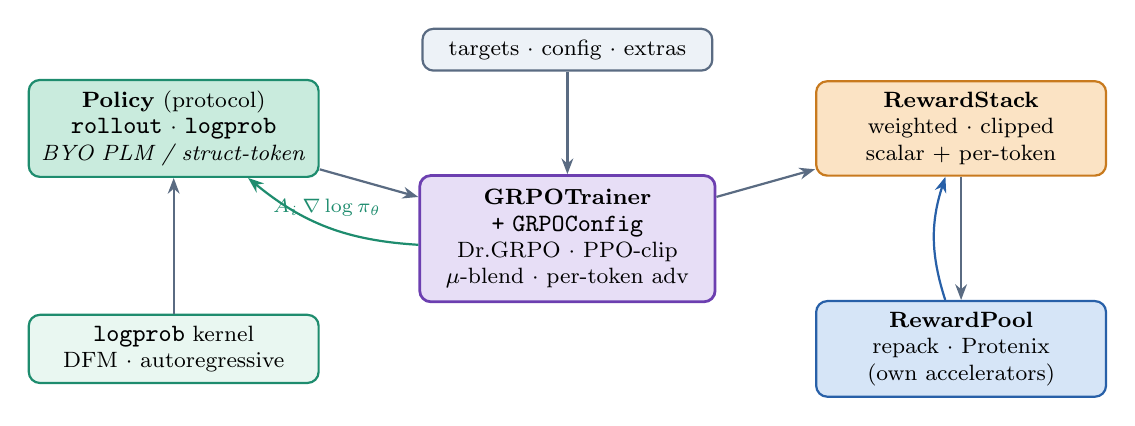
\begin{tikzpicture}[font=\footnotesize,>={Stealth[length=2mm]},
  core/.style={draw=lfLine,fill=lfFill,line width=1.0pt,rounded corners,align=center,inner sep=5pt,text width=3.4cm},
  pol/.style ={draw=aLine,fill=aFill,line width=0.8pt,rounded corners,align=center,inner sep=4pt,text width=3.4cm},
  rw/.style  ={draw=bLine,fill=bFill,line width=0.8pt,rounded corners,align=center,inner sep=4pt,text width=3.4cm},
  io/.style  ={draw=ioLine,fill=ioFill,line width=0.8pt,rounded corners,align=center,inner sep=4pt,text width=3.4cm},
  orc/.style ={draw=dLine,fill=dFill,line width=0.8pt,rounded corners,align=center,inner sep=4pt,text width=3.4cm},
  fl/.style={->,thick,ioLine}]
\node[core] (tr) at (0,0) {\textbf{GRPOTrainer}\\\ttk{+ GRPOConfig}\\Dr.GRPO $\cdot$ PPO-clip\\$\mu$-blend $\cdot$ per-token adv};
\node[pol] (pol) at (-5,1.4) {\textbf{Policy} (protocol)\\\ttk{rollout} $\cdot$ \ttk{logprob}\\\emph{BYO PLM / struct-token}};
\node[pol,fill=aTint] (lp) at (-5,-1.4) {\ttk{logprob} kernel\\DFM $\cdot$ autoregressive};
\node[rw] (rs) at (5,1.4) {\textbf{RewardStack}\\weighted $\cdot$ clipped\\scalar $+$ per-token};
\node[orc] (pool) at (5,-1.4) {\textbf{RewardPool}\\repack $\cdot$ Protenix\\(own accelerators)};
\node[io] (cfg) at (0,2.4) {targets $\cdot$ config $\cdot$ extras};
\draw[fl] (pol) -- (tr);   \draw[fl] (lp) -- (pol);
\draw[fl] (tr) -- (rs);    \draw[fl] (rs) -- (pool);
\draw[fl,dLine] (pool) to[bend left=18] (rs);
\draw[fl] (cfg) -- (tr);
\draw[fl,aLine] (tr) to[bend left=18] node[midway,above,font=\scriptsize]{$A_i\,\nabla\log\pi_\theta$} (pol);
\end{tikzpicture}
\end{center}

\subsection{Scope to ship}
The path is incremental and testable at each step: (1) lift \ttk{rewards} $+$ \ttk{\_dfm\_logprob}
$+$ the queue client into \ttk{plm\_design\_rl} unchanged (they are already pure); (2) extract
\ttk{RewardStack} and the \ttk{GRPOConfig}/optimization half of \ttk{GRPOTrainerConfig} from the
trainer; (3) define the \ttk{Policy}/\ttk{RewardPool} protocols and refactor
\ttk{LeFlurGRPOTrainer} to call them, with an \ttk{adapters/leflur.py} that re-expresses today's
methods as the protocol (regression-tested against the live run for byte-identical rewards and
\ttk{ratio\_init}$\approx1$); (4) publish extras and a \ttk{README} with the two examples above.
Steps 1--2 are pure moves; step 3 is the only real interface work, and the LeFlur adapter is the
proof that the abstraction is faithful.

\end{document}
